% Created by tikzDevice version 0.11 on 2018-07-30 16:04:03
% !TEX encoding = UTF-8 Unicode
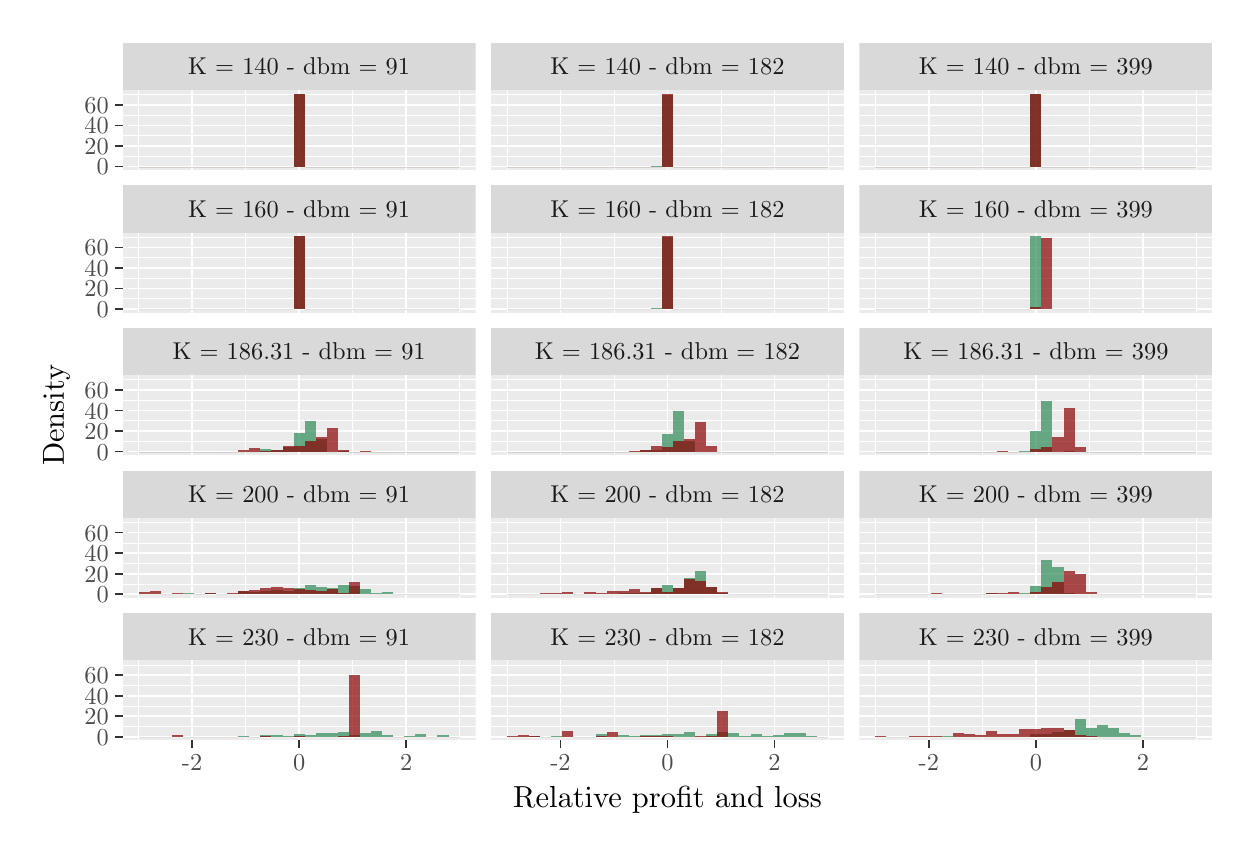
\begin{tikzpicture}[x=1pt,y=1pt]
\definecolor{fillColor}{RGB}{255,255,255}
\path[use as bounding box,fill=fillColor,fill opacity=0.00] (0,0) rectangle (433.62,289.08);
\begin{scope}
\path[clip] (  0.00,  0.00) rectangle (433.62,289.08);
\definecolor{drawColor}{RGB}{255,255,255}
\definecolor{fillColor}{RGB}{255,255,255}

\path[draw=drawColor,line width= 0.6pt,line join=round,line cap=round,fill=fillColor] (  0.00,  0.00) rectangle (433.62,289.08);
\end{scope}
\begin{scope}
\path[clip] ( 34.27,237.57) rectangle (161.89,266.52);
\definecolor{fillColor}{gray}{0.92}

\path[fill=fillColor] ( 34.27,237.57) rectangle (161.89,266.52);
\definecolor{drawColor}{RGB}{255,255,255}

\path[draw=drawColor,line width= 0.3pt,line join=round] ( 34.27,242.59) --
	(161.89,242.59);

\path[draw=drawColor,line width= 0.3pt,line join=round] ( 34.27,250.01) --
	(161.89,250.01);

\path[draw=drawColor,line width= 0.3pt,line join=round] ( 34.27,257.42) --
	(161.89,257.42);

\path[draw=drawColor,line width= 0.3pt,line join=round] ( 34.27,264.83) --
	(161.89,264.83);

\path[draw=drawColor,line width= 0.3pt,line join=round] ( 40.07,237.57) --
	( 40.07,266.52);

\path[draw=drawColor,line width= 0.3pt,line join=round] ( 78.74,237.57) --
	( 78.74,266.52);

\path[draw=drawColor,line width= 0.3pt,line join=round] (117.41,237.57) --
	(117.41,266.52);

\path[draw=drawColor,line width= 0.3pt,line join=round] (156.08,237.57) --
	(156.08,266.52);

\path[draw=drawColor,line width= 0.6pt,line join=round] ( 34.27,238.89) --
	(161.89,238.89);

\path[draw=drawColor,line width= 0.6pt,line join=round] ( 34.27,246.30) --
	(161.89,246.30);

\path[draw=drawColor,line width= 0.6pt,line join=round] ( 34.27,253.71) --
	(161.89,253.71);

\path[draw=drawColor,line width= 0.6pt,line join=round] ( 34.27,261.13) --
	(161.89,261.13);

\path[draw=drawColor,line width= 0.6pt,line join=round] ( 59.40,237.57) --
	( 59.40,266.52);

\path[draw=drawColor,line width= 0.6pt,line join=round] ( 98.08,237.57) --
	( 98.08,266.52);

\path[draw=drawColor,line width= 0.6pt,line join=round] (136.75,237.57) --
	(136.75,266.52);
\definecolor{fillColor}{RGB}{46,139,87}

\path[fill=fillColor,fill opacity=0.70] ( 40.07,238.89) rectangle ( 44.07,238.89);

\path[fill=fillColor,fill opacity=0.70] ( 44.07,238.89) rectangle ( 48.07,238.89);

\path[fill=fillColor,fill opacity=0.70] ( 48.07,238.89) rectangle ( 52.07,238.89);

\path[fill=fillColor,fill opacity=0.70] ( 52.07,238.89) rectangle ( 56.07,238.89);

\path[fill=fillColor,fill opacity=0.70] ( 56.07,238.89) rectangle ( 60.07,238.89);

\path[fill=fillColor,fill opacity=0.70] ( 60.07,238.89) rectangle ( 64.07,238.89);

\path[fill=fillColor,fill opacity=0.70] ( 64.07,238.89) rectangle ( 68.07,238.89);

\path[fill=fillColor,fill opacity=0.70] ( 68.07,238.89) rectangle ( 72.07,238.89);

\path[fill=fillColor,fill opacity=0.70] ( 72.07,238.89) rectangle ( 76.07,238.89);

\path[fill=fillColor,fill opacity=0.70] ( 76.07,238.89) rectangle ( 80.07,238.89);

\path[fill=fillColor,fill opacity=0.70] ( 80.07,238.89) rectangle ( 84.07,238.89);

\path[fill=fillColor,fill opacity=0.70] ( 84.07,238.89) rectangle ( 88.08,238.89);

\path[fill=fillColor,fill opacity=0.70] ( 88.08,238.89) rectangle ( 92.08,238.89);

\path[fill=fillColor,fill opacity=0.70] ( 92.08,238.89) rectangle ( 96.08,238.89);

\path[fill=fillColor,fill opacity=0.70] ( 96.08,238.89) rectangle (100.08,265.20);

\path[fill=fillColor,fill opacity=0.70] (100.08,238.89) rectangle (104.08,238.89);

\path[fill=fillColor,fill opacity=0.70] (104.08,238.89) rectangle (108.08,238.89);

\path[fill=fillColor,fill opacity=0.70] (108.08,238.89) rectangle (112.08,238.89);

\path[fill=fillColor,fill opacity=0.70] (112.08,238.89) rectangle (116.08,238.89);

\path[fill=fillColor,fill opacity=0.70] (116.08,238.89) rectangle (120.08,238.89);

\path[fill=fillColor,fill opacity=0.70] (120.08,238.89) rectangle (124.08,238.89);

\path[fill=fillColor,fill opacity=0.70] (124.08,238.89) rectangle (128.08,238.89);

\path[fill=fillColor,fill opacity=0.70] (128.08,238.89) rectangle (132.08,238.89);

\path[fill=fillColor,fill opacity=0.70] (132.08,238.89) rectangle (136.08,238.89);

\path[fill=fillColor,fill opacity=0.70] (136.08,238.89) rectangle (140.08,238.89);

\path[fill=fillColor,fill opacity=0.70] (140.08,238.89) rectangle (144.08,238.89);

\path[fill=fillColor,fill opacity=0.70] (144.08,238.89) rectangle (148.08,238.89);

\path[fill=fillColor,fill opacity=0.70] (148.08,238.89) rectangle (152.08,238.89);

\path[fill=fillColor,fill opacity=0.70] (152.08,238.89) rectangle (156.08,238.89);
\definecolor{fillColor}{RGB}{139,0,0}

\path[fill=fillColor,fill opacity=0.70] ( 40.07,238.89) rectangle ( 44.07,238.89);

\path[fill=fillColor,fill opacity=0.70] ( 44.07,238.89) rectangle ( 48.07,238.89);

\path[fill=fillColor,fill opacity=0.70] ( 48.07,238.89) rectangle ( 52.07,238.89);

\path[fill=fillColor,fill opacity=0.70] ( 52.07,238.89) rectangle ( 56.07,238.89);

\path[fill=fillColor,fill opacity=0.70] ( 56.07,238.89) rectangle ( 60.07,238.89);

\path[fill=fillColor,fill opacity=0.70] ( 60.07,238.89) rectangle ( 64.07,238.89);

\path[fill=fillColor,fill opacity=0.70] ( 64.07,238.89) rectangle ( 68.07,238.89);

\path[fill=fillColor,fill opacity=0.70] ( 68.07,238.89) rectangle ( 72.07,238.89);

\path[fill=fillColor,fill opacity=0.70] ( 72.07,238.89) rectangle ( 76.07,238.89);

\path[fill=fillColor,fill opacity=0.70] ( 76.07,238.89) rectangle ( 80.07,238.89);

\path[fill=fillColor,fill opacity=0.70] ( 80.07,238.89) rectangle ( 84.07,238.89);

\path[fill=fillColor,fill opacity=0.70] ( 84.07,238.89) rectangle ( 88.08,238.89);

\path[fill=fillColor,fill opacity=0.70] ( 88.08,238.89) rectangle ( 92.08,238.89);

\path[fill=fillColor,fill opacity=0.70] ( 92.08,238.89) rectangle ( 96.08,238.89);

\path[fill=fillColor,fill opacity=0.70] ( 96.08,238.89) rectangle (100.08,265.20);

\path[fill=fillColor,fill opacity=0.70] (100.08,238.89) rectangle (104.08,238.89);

\path[fill=fillColor,fill opacity=0.70] (104.08,238.89) rectangle (108.08,238.89);

\path[fill=fillColor,fill opacity=0.70] (108.08,238.89) rectangle (112.08,238.89);

\path[fill=fillColor,fill opacity=0.70] (112.08,238.89) rectangle (116.08,238.89);

\path[fill=fillColor,fill opacity=0.70] (116.08,238.89) rectangle (120.08,238.89);

\path[fill=fillColor,fill opacity=0.70] (120.08,238.89) rectangle (124.08,238.89);

\path[fill=fillColor,fill opacity=0.70] (124.08,238.89) rectangle (128.08,238.89);

\path[fill=fillColor,fill opacity=0.70] (128.08,238.89) rectangle (132.08,238.89);

\path[fill=fillColor,fill opacity=0.70] (132.08,238.89) rectangle (136.08,238.89);

\path[fill=fillColor,fill opacity=0.70] (136.08,238.89) rectangle (140.08,238.89);

\path[fill=fillColor,fill opacity=0.70] (140.08,238.89) rectangle (144.08,238.89);

\path[fill=fillColor,fill opacity=0.70] (144.08,238.89) rectangle (148.08,238.89);

\path[fill=fillColor,fill opacity=0.70] (148.08,238.89) rectangle (152.08,238.89);

\path[fill=fillColor,fill opacity=0.70] (152.08,238.89) rectangle (156.08,238.89);
\end{scope}
\begin{scope}
\path[clip] ( 34.27,186.06) rectangle (161.89,215.01);
\definecolor{fillColor}{gray}{0.92}

\path[fill=fillColor] ( 34.27,186.06) rectangle (161.89,215.01);
\definecolor{drawColor}{RGB}{255,255,255}

\path[draw=drawColor,line width= 0.3pt,line join=round] ( 34.27,191.08) --
	(161.89,191.08);

\path[draw=drawColor,line width= 0.3pt,line join=round] ( 34.27,198.50) --
	(161.89,198.50);

\path[draw=drawColor,line width= 0.3pt,line join=round] ( 34.27,205.91) --
	(161.89,205.91);

\path[draw=drawColor,line width= 0.3pt,line join=round] ( 34.27,213.32) --
	(161.89,213.32);

\path[draw=drawColor,line width= 0.3pt,line join=round] ( 40.07,186.06) --
	( 40.07,215.01);

\path[draw=drawColor,line width= 0.3pt,line join=round] ( 78.74,186.06) --
	( 78.74,215.01);

\path[draw=drawColor,line width= 0.3pt,line join=round] (117.41,186.06) --
	(117.41,215.01);

\path[draw=drawColor,line width= 0.3pt,line join=round] (156.08,186.06) --
	(156.08,215.01);

\path[draw=drawColor,line width= 0.6pt,line join=round] ( 34.27,187.38) --
	(161.89,187.38);

\path[draw=drawColor,line width= 0.6pt,line join=round] ( 34.27,194.79) --
	(161.89,194.79);

\path[draw=drawColor,line width= 0.6pt,line join=round] ( 34.27,202.20) --
	(161.89,202.20);

\path[draw=drawColor,line width= 0.6pt,line join=round] ( 34.27,209.62) --
	(161.89,209.62);

\path[draw=drawColor,line width= 0.6pt,line join=round] ( 59.40,186.06) --
	( 59.40,215.01);

\path[draw=drawColor,line width= 0.6pt,line join=round] ( 98.08,186.06) --
	( 98.08,215.01);

\path[draw=drawColor,line width= 0.6pt,line join=round] (136.75,186.06) --
	(136.75,215.01);
\definecolor{fillColor}{RGB}{46,139,87}

\path[fill=fillColor,fill opacity=0.70] ( 40.07,187.38) rectangle ( 44.07,187.38);

\path[fill=fillColor,fill opacity=0.70] ( 44.07,187.38) rectangle ( 48.07,187.38);

\path[fill=fillColor,fill opacity=0.70] ( 48.07,187.38) rectangle ( 52.07,187.38);

\path[fill=fillColor,fill opacity=0.70] ( 52.07,187.38) rectangle ( 56.07,187.38);

\path[fill=fillColor,fill opacity=0.70] ( 56.07,187.38) rectangle ( 60.07,187.38);

\path[fill=fillColor,fill opacity=0.70] ( 60.07,187.38) rectangle ( 64.07,187.38);

\path[fill=fillColor,fill opacity=0.70] ( 64.07,187.38) rectangle ( 68.07,187.38);

\path[fill=fillColor,fill opacity=0.70] ( 68.07,187.38) rectangle ( 72.07,187.38);

\path[fill=fillColor,fill opacity=0.70] ( 72.07,187.38) rectangle ( 76.07,187.38);

\path[fill=fillColor,fill opacity=0.70] ( 76.07,187.38) rectangle ( 80.07,187.38);

\path[fill=fillColor,fill opacity=0.70] ( 80.07,187.38) rectangle ( 84.07,187.38);

\path[fill=fillColor,fill opacity=0.70] ( 84.07,187.38) rectangle ( 88.08,187.38);

\path[fill=fillColor,fill opacity=0.70] ( 88.08,187.38) rectangle ( 92.08,187.38);

\path[fill=fillColor,fill opacity=0.70] ( 92.08,187.38) rectangle ( 96.08,187.38);

\path[fill=fillColor,fill opacity=0.70] ( 96.08,187.38) rectangle (100.08,213.69);

\path[fill=fillColor,fill opacity=0.70] (100.08,187.38) rectangle (104.08,187.38);

\path[fill=fillColor,fill opacity=0.70] (104.08,187.38) rectangle (108.08,187.38);

\path[fill=fillColor,fill opacity=0.70] (108.08,187.38) rectangle (112.08,187.38);

\path[fill=fillColor,fill opacity=0.70] (112.08,187.38) rectangle (116.08,187.38);

\path[fill=fillColor,fill opacity=0.70] (116.08,187.38) rectangle (120.08,187.38);

\path[fill=fillColor,fill opacity=0.70] (120.08,187.38) rectangle (124.08,187.38);

\path[fill=fillColor,fill opacity=0.70] (124.08,187.38) rectangle (128.08,187.38);

\path[fill=fillColor,fill opacity=0.70] (128.08,187.38) rectangle (132.08,187.38);

\path[fill=fillColor,fill opacity=0.70] (132.08,187.38) rectangle (136.08,187.38);

\path[fill=fillColor,fill opacity=0.70] (136.08,187.38) rectangle (140.08,187.38);

\path[fill=fillColor,fill opacity=0.70] (140.08,187.38) rectangle (144.08,187.38);

\path[fill=fillColor,fill opacity=0.70] (144.08,187.38) rectangle (148.08,187.38);

\path[fill=fillColor,fill opacity=0.70] (148.08,187.38) rectangle (152.08,187.38);

\path[fill=fillColor,fill opacity=0.70] (152.08,187.38) rectangle (156.08,187.38);
\definecolor{fillColor}{RGB}{139,0,0}

\path[fill=fillColor,fill opacity=0.70] ( 40.07,187.38) rectangle ( 44.07,187.38);

\path[fill=fillColor,fill opacity=0.70] ( 44.07,187.38) rectangle ( 48.07,187.38);

\path[fill=fillColor,fill opacity=0.70] ( 48.07,187.38) rectangle ( 52.07,187.38);

\path[fill=fillColor,fill opacity=0.70] ( 52.07,187.38) rectangle ( 56.07,187.38);

\path[fill=fillColor,fill opacity=0.70] ( 56.07,187.38) rectangle ( 60.07,187.38);

\path[fill=fillColor,fill opacity=0.70] ( 60.07,187.38) rectangle ( 64.07,187.38);

\path[fill=fillColor,fill opacity=0.70] ( 64.07,187.38) rectangle ( 68.07,187.38);

\path[fill=fillColor,fill opacity=0.70] ( 68.07,187.38) rectangle ( 72.07,187.38);

\path[fill=fillColor,fill opacity=0.70] ( 72.07,187.38) rectangle ( 76.07,187.38);

\path[fill=fillColor,fill opacity=0.70] ( 76.07,187.38) rectangle ( 80.07,187.38);

\path[fill=fillColor,fill opacity=0.70] ( 80.07,187.38) rectangle ( 84.07,187.38);

\path[fill=fillColor,fill opacity=0.70] ( 84.07,187.38) rectangle ( 88.08,187.38);

\path[fill=fillColor,fill opacity=0.70] ( 88.08,187.38) rectangle ( 92.08,187.38);

\path[fill=fillColor,fill opacity=0.70] ( 92.08,187.38) rectangle ( 96.08,187.38);

\path[fill=fillColor,fill opacity=0.70] ( 96.08,187.38) rectangle (100.08,213.69);

\path[fill=fillColor,fill opacity=0.70] (100.08,187.38) rectangle (104.08,187.38);

\path[fill=fillColor,fill opacity=0.70] (104.08,187.38) rectangle (108.08,187.38);

\path[fill=fillColor,fill opacity=0.70] (108.08,187.38) rectangle (112.08,187.38);

\path[fill=fillColor,fill opacity=0.70] (112.08,187.38) rectangle (116.08,187.38);

\path[fill=fillColor,fill opacity=0.70] (116.08,187.38) rectangle (120.08,187.38);

\path[fill=fillColor,fill opacity=0.70] (120.08,187.38) rectangle (124.08,187.38);

\path[fill=fillColor,fill opacity=0.70] (124.08,187.38) rectangle (128.08,187.38);

\path[fill=fillColor,fill opacity=0.70] (128.08,187.38) rectangle (132.08,187.38);

\path[fill=fillColor,fill opacity=0.70] (132.08,187.38) rectangle (136.08,187.38);

\path[fill=fillColor,fill opacity=0.70] (136.08,187.38) rectangle (140.08,187.38);

\path[fill=fillColor,fill opacity=0.70] (140.08,187.38) rectangle (144.08,187.38);

\path[fill=fillColor,fill opacity=0.70] (144.08,187.38) rectangle (148.08,187.38);

\path[fill=fillColor,fill opacity=0.70] (148.08,187.38) rectangle (152.08,187.38);

\path[fill=fillColor,fill opacity=0.70] (152.08,187.38) rectangle (156.08,187.38);
\end{scope}
\begin{scope}
\path[clip] ( 34.27,134.55) rectangle (161.89,163.50);
\definecolor{fillColor}{gray}{0.92}

\path[fill=fillColor] ( 34.27,134.55) rectangle (161.89,163.50);
\definecolor{drawColor}{RGB}{255,255,255}

\path[draw=drawColor,line width= 0.3pt,line join=round] ( 34.27,139.57) --
	(161.89,139.57);

\path[draw=drawColor,line width= 0.3pt,line join=round] ( 34.27,146.99) --
	(161.89,146.99);

\path[draw=drawColor,line width= 0.3pt,line join=round] ( 34.27,154.40) --
	(161.89,154.40);

\path[draw=drawColor,line width= 0.3pt,line join=round] ( 34.27,161.81) --
	(161.89,161.81);

\path[draw=drawColor,line width= 0.3pt,line join=round] ( 40.07,134.55) --
	( 40.07,163.50);

\path[draw=drawColor,line width= 0.3pt,line join=round] ( 78.74,134.55) --
	( 78.74,163.50);

\path[draw=drawColor,line width= 0.3pt,line join=round] (117.41,134.55) --
	(117.41,163.50);

\path[draw=drawColor,line width= 0.3pt,line join=round] (156.08,134.55) --
	(156.08,163.50);

\path[draw=drawColor,line width= 0.6pt,line join=round] ( 34.27,135.87) --
	(161.89,135.87);

\path[draw=drawColor,line width= 0.6pt,line join=round] ( 34.27,143.28) --
	(161.89,143.28);

\path[draw=drawColor,line width= 0.6pt,line join=round] ( 34.27,150.69) --
	(161.89,150.69);

\path[draw=drawColor,line width= 0.6pt,line join=round] ( 34.27,158.11) --
	(161.89,158.11);

\path[draw=drawColor,line width= 0.6pt,line join=round] ( 59.40,134.55) --
	( 59.40,163.50);

\path[draw=drawColor,line width= 0.6pt,line join=round] ( 98.08,134.55) --
	( 98.08,163.50);

\path[draw=drawColor,line width= 0.6pt,line join=round] (136.75,134.55) --
	(136.75,163.50);
\definecolor{fillColor}{RGB}{46,139,87}

\path[fill=fillColor,fill opacity=0.70] ( 40.07,135.87) rectangle ( 44.07,135.87);

\path[fill=fillColor,fill opacity=0.70] ( 44.07,135.87) rectangle ( 48.07,135.87);

\path[fill=fillColor,fill opacity=0.70] ( 48.07,135.87) rectangle ( 52.07,135.87);

\path[fill=fillColor,fill opacity=0.70] ( 52.07,135.87) rectangle ( 56.07,135.87);

\path[fill=fillColor,fill opacity=0.70] ( 56.07,135.87) rectangle ( 60.07,135.87);

\path[fill=fillColor,fill opacity=0.70] ( 60.07,135.87) rectangle ( 64.07,135.87);

\path[fill=fillColor,fill opacity=0.70] ( 64.07,135.87) rectangle ( 68.07,135.87);

\path[fill=fillColor,fill opacity=0.70] ( 68.07,135.87) rectangle ( 72.07,135.87);

\path[fill=fillColor,fill opacity=0.70] ( 72.07,135.87) rectangle ( 76.07,135.87);

\path[fill=fillColor,fill opacity=0.70] ( 76.07,135.87) rectangle ( 80.07,135.87);

\path[fill=fillColor,fill opacity=0.70] ( 80.07,135.87) rectangle ( 84.07,135.87);

\path[fill=fillColor,fill opacity=0.70] ( 84.07,135.87) rectangle ( 88.08,136.98);

\path[fill=fillColor,fill opacity=0.70] ( 88.08,135.87) rectangle ( 92.08,136.61);

\path[fill=fillColor,fill opacity=0.70] ( 92.08,135.87) rectangle ( 96.08,137.72);

\path[fill=fillColor,fill opacity=0.70] ( 96.08,135.87) rectangle (100.08,142.54);

\path[fill=fillColor,fill opacity=0.70] (100.08,135.87) rectangle (104.08,146.99);

\path[fill=fillColor,fill opacity=0.70] (104.08,135.87) rectangle (108.08,140.31);

\path[fill=fillColor,fill opacity=0.70] (108.08,135.87) rectangle (112.08,135.87);

\path[fill=fillColor,fill opacity=0.70] (112.08,135.87) rectangle (116.08,136.24);

\path[fill=fillColor,fill opacity=0.70] (116.08,135.87) rectangle (120.08,135.87);

\path[fill=fillColor,fill opacity=0.70] (120.08,135.87) rectangle (124.08,135.87);

\path[fill=fillColor,fill opacity=0.70] (124.08,135.87) rectangle (128.08,135.87);

\path[fill=fillColor,fill opacity=0.70] (128.08,135.87) rectangle (132.08,135.87);

\path[fill=fillColor,fill opacity=0.70] (132.08,135.87) rectangle (136.08,135.87);

\path[fill=fillColor,fill opacity=0.70] (136.08,135.87) rectangle (140.08,135.87);

\path[fill=fillColor,fill opacity=0.70] (140.08,135.87) rectangle (144.08,135.87);

\path[fill=fillColor,fill opacity=0.70] (144.08,135.87) rectangle (148.08,135.87);

\path[fill=fillColor,fill opacity=0.70] (148.08,135.87) rectangle (152.08,135.87);

\path[fill=fillColor,fill opacity=0.70] (152.08,135.87) rectangle (156.08,135.87);
\definecolor{fillColor}{RGB}{139,0,0}

\path[fill=fillColor,fill opacity=0.70] ( 40.07,135.87) rectangle ( 44.07,135.87);

\path[fill=fillColor,fill opacity=0.70] ( 44.07,135.87) rectangle ( 48.07,135.87);

\path[fill=fillColor,fill opacity=0.70] ( 48.07,135.87) rectangle ( 52.07,135.87);

\path[fill=fillColor,fill opacity=0.70] ( 52.07,135.87) rectangle ( 56.07,135.87);

\path[fill=fillColor,fill opacity=0.70] ( 56.07,135.87) rectangle ( 60.07,135.87);

\path[fill=fillColor,fill opacity=0.70] ( 60.07,135.87) rectangle ( 64.07,135.87);

\path[fill=fillColor,fill opacity=0.70] ( 64.07,135.87) rectangle ( 68.07,135.87);

\path[fill=fillColor,fill opacity=0.70] ( 68.07,135.87) rectangle ( 72.07,135.87);

\path[fill=fillColor,fill opacity=0.70] ( 72.07,135.87) rectangle ( 76.07,135.87);

\path[fill=fillColor,fill opacity=0.70] ( 76.07,135.87) rectangle ( 80.07,136.61);

\path[fill=fillColor,fill opacity=0.70] ( 80.07,135.87) rectangle ( 84.07,137.35);

\path[fill=fillColor,fill opacity=0.70] ( 84.07,135.87) rectangle ( 88.08,136.24);

\path[fill=fillColor,fill opacity=0.70] ( 88.08,135.87) rectangle ( 92.08,136.61);

\path[fill=fillColor,fill opacity=0.70] ( 92.08,135.87) rectangle ( 96.08,138.09);

\path[fill=fillColor,fill opacity=0.70] ( 96.08,135.87) rectangle (100.08,138.09);

\path[fill=fillColor,fill opacity=0.70] (100.08,135.87) rectangle (104.08,139.57);

\path[fill=fillColor,fill opacity=0.70] (104.08,135.87) rectangle (108.08,141.06);

\path[fill=fillColor,fill opacity=0.70] (108.08,135.87) rectangle (112.08,144.39);

\path[fill=fillColor,fill opacity=0.70] (112.08,135.87) rectangle (116.08,136.61);

\path[fill=fillColor,fill opacity=0.70] (116.08,135.87) rectangle (120.08,135.87);

\path[fill=fillColor,fill opacity=0.70] (120.08,135.87) rectangle (124.08,136.24);

\path[fill=fillColor,fill opacity=0.70] (124.08,135.87) rectangle (128.08,135.87);

\path[fill=fillColor,fill opacity=0.70] (128.08,135.87) rectangle (132.08,135.87);

\path[fill=fillColor,fill opacity=0.70] (132.08,135.87) rectangle (136.08,135.87);

\path[fill=fillColor,fill opacity=0.70] (136.08,135.87) rectangle (140.08,135.87);

\path[fill=fillColor,fill opacity=0.70] (140.08,135.87) rectangle (144.08,135.87);

\path[fill=fillColor,fill opacity=0.70] (144.08,135.87) rectangle (148.08,135.87);

\path[fill=fillColor,fill opacity=0.70] (148.08,135.87) rectangle (152.08,135.87);

\path[fill=fillColor,fill opacity=0.70] (152.08,135.87) rectangle (156.08,135.87);
\end{scope}
\begin{scope}
\path[clip] ( 34.27, 83.04) rectangle (161.89,111.99);
\definecolor{fillColor}{gray}{0.92}

\path[fill=fillColor] ( 34.27, 83.04) rectangle (161.89,111.99);
\definecolor{drawColor}{RGB}{255,255,255}

\path[draw=drawColor,line width= 0.3pt,line join=round] ( 34.27, 88.06) --
	(161.89, 88.06);

\path[draw=drawColor,line width= 0.3pt,line join=round] ( 34.27, 95.48) --
	(161.89, 95.48);

\path[draw=drawColor,line width= 0.3pt,line join=round] ( 34.27,102.89) --
	(161.89,102.89);

\path[draw=drawColor,line width= 0.3pt,line join=round] ( 34.27,110.30) --
	(161.89,110.30);

\path[draw=drawColor,line width= 0.3pt,line join=round] ( 40.07, 83.04) --
	( 40.07,111.99);

\path[draw=drawColor,line width= 0.3pt,line join=round] ( 78.74, 83.04) --
	( 78.74,111.99);

\path[draw=drawColor,line width= 0.3pt,line join=round] (117.41, 83.04) --
	(117.41,111.99);

\path[draw=drawColor,line width= 0.3pt,line join=round] (156.08, 83.04) --
	(156.08,111.99);

\path[draw=drawColor,line width= 0.6pt,line join=round] ( 34.27, 84.36) --
	(161.89, 84.36);

\path[draw=drawColor,line width= 0.6pt,line join=round] ( 34.27, 91.77) --
	(161.89, 91.77);

\path[draw=drawColor,line width= 0.6pt,line join=round] ( 34.27, 99.18) --
	(161.89, 99.18);

\path[draw=drawColor,line width= 0.6pt,line join=round] ( 34.27,106.60) --
	(161.89,106.60);

\path[draw=drawColor,line width= 0.6pt,line join=round] ( 59.40, 83.04) --
	( 59.40,111.99);

\path[draw=drawColor,line width= 0.6pt,line join=round] ( 98.08, 83.04) --
	( 98.08,111.99);

\path[draw=drawColor,line width= 0.6pt,line join=round] (136.75, 83.04) --
	(136.75,111.99);
\definecolor{fillColor}{RGB}{46,139,87}

\path[fill=fillColor,fill opacity=0.70] ( 40.07, 84.36) rectangle ( 44.07, 84.36);

\path[fill=fillColor,fill opacity=0.70] ( 44.07, 84.36) rectangle ( 48.07, 84.36);

\path[fill=fillColor,fill opacity=0.70] ( 48.07, 84.36) rectangle ( 52.07, 84.36);

\path[fill=fillColor,fill opacity=0.70] ( 52.07, 84.36) rectangle ( 56.07, 84.36);

\path[fill=fillColor,fill opacity=0.70] ( 56.07, 84.36) rectangle ( 60.07, 84.73);

\path[fill=fillColor,fill opacity=0.70] ( 60.07, 84.36) rectangle ( 64.07, 84.36);

\path[fill=fillColor,fill opacity=0.70] ( 64.07, 84.36) rectangle ( 68.07, 84.73);

\path[fill=fillColor,fill opacity=0.70] ( 68.07, 84.36) rectangle ( 72.07, 84.36);

\path[fill=fillColor,fill opacity=0.70] ( 72.07, 84.36) rectangle ( 76.07, 84.36);

\path[fill=fillColor,fill opacity=0.70] ( 76.07, 84.36) rectangle ( 80.07, 85.47);

\path[fill=fillColor,fill opacity=0.70] ( 80.07, 84.36) rectangle ( 84.07, 85.10);

\path[fill=fillColor,fill opacity=0.70] ( 84.07, 84.36) rectangle ( 88.08, 85.47);

\path[fill=fillColor,fill opacity=0.70] ( 88.08, 84.36) rectangle ( 92.08, 85.84);

\path[fill=fillColor,fill opacity=0.70] ( 92.08, 84.36) rectangle ( 96.08, 85.47);

\path[fill=fillColor,fill opacity=0.70] ( 96.08, 84.36) rectangle (100.08, 86.58);

\path[fill=fillColor,fill opacity=0.70] (100.08, 84.36) rectangle (104.08, 87.69);

\path[fill=fillColor,fill opacity=0.70] (104.08, 84.36) rectangle (108.08, 86.95);

\path[fill=fillColor,fill opacity=0.70] (108.08, 84.36) rectangle (112.08, 86.58);

\path[fill=fillColor,fill opacity=0.70] (112.08, 84.36) rectangle (116.08, 87.69);

\path[fill=fillColor,fill opacity=0.70] (116.08, 84.36) rectangle (120.08, 87.32);

\path[fill=fillColor,fill opacity=0.70] (120.08, 84.36) rectangle (124.08, 86.21);

\path[fill=fillColor,fill opacity=0.70] (124.08, 84.36) rectangle (128.08, 84.73);

\path[fill=fillColor,fill opacity=0.70] (128.08, 84.36) rectangle (132.08, 85.10);

\path[fill=fillColor,fill opacity=0.70] (132.08, 84.36) rectangle (136.08, 84.36);

\path[fill=fillColor,fill opacity=0.70] (136.08, 84.36) rectangle (140.08, 84.36);

\path[fill=fillColor,fill opacity=0.70] (140.08, 84.36) rectangle (144.08, 84.36);

\path[fill=fillColor,fill opacity=0.70] (144.08, 84.36) rectangle (148.08, 84.36);

\path[fill=fillColor,fill opacity=0.70] (148.08, 84.36) rectangle (152.08, 84.36);

\path[fill=fillColor,fill opacity=0.70] (152.08, 84.36) rectangle (156.08, 84.36);
\definecolor{fillColor}{RGB}{139,0,0}

\path[fill=fillColor,fill opacity=0.70] ( 40.07, 84.36) rectangle ( 44.07, 85.10);

\path[fill=fillColor,fill opacity=0.70] ( 44.07, 84.36) rectangle ( 48.07, 85.47);

\path[fill=fillColor,fill opacity=0.70] ( 48.07, 84.36) rectangle ( 52.07, 84.36);

\path[fill=fillColor,fill opacity=0.70] ( 52.07, 84.36) rectangle ( 56.07, 84.73);

\path[fill=fillColor,fill opacity=0.70] ( 56.07, 84.36) rectangle ( 60.07, 84.36);

\path[fill=fillColor,fill opacity=0.70] ( 60.07, 84.36) rectangle ( 64.07, 84.36);

\path[fill=fillColor,fill opacity=0.70] ( 64.07, 84.36) rectangle ( 68.07, 84.73);

\path[fill=fillColor,fill opacity=0.70] ( 68.07, 84.36) rectangle ( 72.07, 84.36);

\path[fill=fillColor,fill opacity=0.70] ( 72.07, 84.36) rectangle ( 76.07, 84.73);

\path[fill=fillColor,fill opacity=0.70] ( 76.07, 84.36) rectangle ( 80.07, 85.47);

\path[fill=fillColor,fill opacity=0.70] ( 80.07, 84.36) rectangle ( 84.07, 85.84);

\path[fill=fillColor,fill opacity=0.70] ( 84.07, 84.36) rectangle ( 88.08, 86.58);

\path[fill=fillColor,fill opacity=0.70] ( 88.08, 84.36) rectangle ( 92.08, 86.95);

\path[fill=fillColor,fill opacity=0.70] ( 92.08, 84.36) rectangle ( 96.08, 86.58);

\path[fill=fillColor,fill opacity=0.70] ( 96.08, 84.36) rectangle (100.08, 86.21);

\path[fill=fillColor,fill opacity=0.70] (100.08, 84.36) rectangle (104.08, 85.84);

\path[fill=fillColor,fill opacity=0.70] (104.08, 84.36) rectangle (108.08, 85.47);

\path[fill=fillColor,fill opacity=0.70] (108.08, 84.36) rectangle (112.08, 86.21);

\path[fill=fillColor,fill opacity=0.70] (112.08, 84.36) rectangle (116.08, 84.73);

\path[fill=fillColor,fill opacity=0.70] (116.08, 84.36) rectangle (120.08, 88.80);

\path[fill=fillColor,fill opacity=0.70] (120.08, 84.36) rectangle (124.08, 84.36);

\path[fill=fillColor,fill opacity=0.70] (124.08, 84.36) rectangle (128.08, 84.36);

\path[fill=fillColor,fill opacity=0.70] (128.08, 84.36) rectangle (132.08, 84.36);

\path[fill=fillColor,fill opacity=0.70] (132.08, 84.36) rectangle (136.08, 84.36);

\path[fill=fillColor,fill opacity=0.70] (136.08, 84.36) rectangle (140.08, 84.36);

\path[fill=fillColor,fill opacity=0.70] (140.08, 84.36) rectangle (144.08, 84.36);

\path[fill=fillColor,fill opacity=0.70] (144.08, 84.36) rectangle (148.08, 84.36);

\path[fill=fillColor,fill opacity=0.70] (148.08, 84.36) rectangle (152.08, 84.36);

\path[fill=fillColor,fill opacity=0.70] (152.08, 84.36) rectangle (156.08, 84.36);
\end{scope}
\begin{scope}
\path[clip] ( 34.27, 31.53) rectangle (161.89, 60.48);
\definecolor{fillColor}{gray}{0.92}

\path[fill=fillColor] ( 34.27, 31.53) rectangle (161.89, 60.48);
\definecolor{drawColor}{RGB}{255,255,255}

\path[draw=drawColor,line width= 0.3pt,line join=round] ( 34.27, 36.55) --
	(161.89, 36.55);

\path[draw=drawColor,line width= 0.3pt,line join=round] ( 34.27, 43.97) --
	(161.89, 43.97);

\path[draw=drawColor,line width= 0.3pt,line join=round] ( 34.27, 51.38) --
	(161.89, 51.38);

\path[draw=drawColor,line width= 0.3pt,line join=round] ( 34.27, 58.79) --
	(161.89, 58.79);

\path[draw=drawColor,line width= 0.3pt,line join=round] ( 40.07, 31.53) --
	( 40.07, 60.48);

\path[draw=drawColor,line width= 0.3pt,line join=round] ( 78.74, 31.53) --
	( 78.74, 60.48);

\path[draw=drawColor,line width= 0.3pt,line join=round] (117.41, 31.53) --
	(117.41, 60.48);

\path[draw=drawColor,line width= 0.3pt,line join=round] (156.08, 31.53) --
	(156.08, 60.48);

\path[draw=drawColor,line width= 0.6pt,line join=round] ( 34.27, 32.85) --
	(161.89, 32.85);

\path[draw=drawColor,line width= 0.6pt,line join=round] ( 34.27, 40.26) --
	(161.89, 40.26);

\path[draw=drawColor,line width= 0.6pt,line join=round] ( 34.27, 47.67) --
	(161.89, 47.67);

\path[draw=drawColor,line width= 0.6pt,line join=round] ( 34.27, 55.09) --
	(161.89, 55.09);

\path[draw=drawColor,line width= 0.6pt,line join=round] ( 59.40, 31.53) --
	( 59.40, 60.48);

\path[draw=drawColor,line width= 0.6pt,line join=round] ( 98.08, 31.53) --
	( 98.08, 60.48);

\path[draw=drawColor,line width= 0.6pt,line join=round] (136.75, 31.53) --
	(136.75, 60.48);
\definecolor{fillColor}{RGB}{46,139,87}

\path[fill=fillColor,fill opacity=0.70] ( 40.07, 32.85) rectangle ( 44.07, 32.85);

\path[fill=fillColor,fill opacity=0.70] ( 44.07, 32.85) rectangle ( 48.07, 32.85);

\path[fill=fillColor,fill opacity=0.70] ( 48.07, 32.85) rectangle ( 52.07, 32.85);

\path[fill=fillColor,fill opacity=0.70] ( 52.07, 32.85) rectangle ( 56.07, 32.85);

\path[fill=fillColor,fill opacity=0.70] ( 56.07, 32.85) rectangle ( 60.07, 32.85);

\path[fill=fillColor,fill opacity=0.70] ( 60.07, 32.85) rectangle ( 64.07, 32.85);

\path[fill=fillColor,fill opacity=0.70] ( 64.07, 32.85) rectangle ( 68.07, 32.85);

\path[fill=fillColor,fill opacity=0.70] ( 68.07, 32.85) rectangle ( 72.07, 32.85);

\path[fill=fillColor,fill opacity=0.70] ( 72.07, 32.85) rectangle ( 76.07, 32.85);

\path[fill=fillColor,fill opacity=0.70] ( 76.07, 32.85) rectangle ( 80.07, 33.22);

\path[fill=fillColor,fill opacity=0.70] ( 80.07, 32.85) rectangle ( 84.07, 32.85);

\path[fill=fillColor,fill opacity=0.70] ( 84.07, 32.85) rectangle ( 88.08, 33.59);

\path[fill=fillColor,fill opacity=0.70] ( 88.08, 32.85) rectangle ( 92.08, 33.59);

\path[fill=fillColor,fill opacity=0.70] ( 92.08, 32.85) rectangle ( 96.08, 33.22);

\path[fill=fillColor,fill opacity=0.70] ( 96.08, 32.85) rectangle (100.08, 33.96);

\path[fill=fillColor,fill opacity=0.70] (100.08, 32.85) rectangle (104.08, 33.59);

\path[fill=fillColor,fill opacity=0.70] (104.08, 32.85) rectangle (108.08, 34.33);

\path[fill=fillColor,fill opacity=0.70] (108.08, 32.85) rectangle (112.08, 34.33);

\path[fill=fillColor,fill opacity=0.70] (112.08, 32.85) rectangle (116.08, 34.70);

\path[fill=fillColor,fill opacity=0.70] (116.08, 32.85) rectangle (120.08, 33.59);

\path[fill=fillColor,fill opacity=0.70] (120.08, 32.85) rectangle (124.08, 34.33);

\path[fill=fillColor,fill opacity=0.70] (124.08, 32.85) rectangle (128.08, 35.07);

\path[fill=fillColor,fill opacity=0.70] (128.08, 32.85) rectangle (132.08, 33.59);

\path[fill=fillColor,fill opacity=0.70] (132.08, 32.85) rectangle (136.08, 32.85);

\path[fill=fillColor,fill opacity=0.70] (136.08, 32.85) rectangle (140.08, 33.22);

\path[fill=fillColor,fill opacity=0.70] (140.08, 32.85) rectangle (144.08, 33.96);

\path[fill=fillColor,fill opacity=0.70] (144.08, 32.85) rectangle (148.08, 32.85);

\path[fill=fillColor,fill opacity=0.70] (148.08, 32.85) rectangle (152.08, 33.59);

\path[fill=fillColor,fill opacity=0.70] (152.08, 32.85) rectangle (156.08, 32.85);
\definecolor{fillColor}{RGB}{139,0,0}

\path[fill=fillColor,fill opacity=0.70] ( 40.07, 32.85) rectangle ( 44.07, 32.85);

\path[fill=fillColor,fill opacity=0.70] ( 44.07, 32.85) rectangle ( 48.07, 32.85);

\path[fill=fillColor,fill opacity=0.70] ( 48.07, 32.85) rectangle ( 52.07, 32.85);

\path[fill=fillColor,fill opacity=0.70] ( 52.07, 32.85) rectangle ( 56.07, 33.59);

\path[fill=fillColor,fill opacity=0.70] ( 56.07, 32.85) rectangle ( 60.07, 32.85);

\path[fill=fillColor,fill opacity=0.70] ( 60.07, 32.85) rectangle ( 64.07, 32.85);

\path[fill=fillColor,fill opacity=0.70] ( 64.07, 32.85) rectangle ( 68.07, 32.85);

\path[fill=fillColor,fill opacity=0.70] ( 68.07, 32.85) rectangle ( 72.07, 32.85);

\path[fill=fillColor,fill opacity=0.70] ( 72.07, 32.85) rectangle ( 76.07, 32.85);

\path[fill=fillColor,fill opacity=0.70] ( 76.07, 32.85) rectangle ( 80.07, 32.85);

\path[fill=fillColor,fill opacity=0.70] ( 80.07, 32.85) rectangle ( 84.07, 32.85);

\path[fill=fillColor,fill opacity=0.70] ( 84.07, 32.85) rectangle ( 88.08, 33.22);

\path[fill=fillColor,fill opacity=0.70] ( 88.08, 32.85) rectangle ( 92.08, 32.85);

\path[fill=fillColor,fill opacity=0.70] ( 92.08, 32.85) rectangle ( 96.08, 32.85);

\path[fill=fillColor,fill opacity=0.70] ( 96.08, 32.85) rectangle (100.08, 33.22);

\path[fill=fillColor,fill opacity=0.70] (100.08, 32.85) rectangle (104.08, 32.85);

\path[fill=fillColor,fill opacity=0.70] (104.08, 32.85) rectangle (108.08, 32.85);

\path[fill=fillColor,fill opacity=0.70] (108.08, 32.85) rectangle (112.08, 32.85);

\path[fill=fillColor,fill opacity=0.70] (112.08, 32.85) rectangle (116.08, 33.22);

\path[fill=fillColor,fill opacity=0.70] (116.08, 32.85) rectangle (120.08, 55.09);

\path[fill=fillColor,fill opacity=0.70] (120.08, 32.85) rectangle (124.08, 32.85);

\path[fill=fillColor,fill opacity=0.70] (124.08, 32.85) rectangle (128.08, 32.85);

\path[fill=fillColor,fill opacity=0.70] (128.08, 32.85) rectangle (132.08, 32.85);

\path[fill=fillColor,fill opacity=0.70] (132.08, 32.85) rectangle (136.08, 32.85);

\path[fill=fillColor,fill opacity=0.70] (136.08, 32.85) rectangle (140.08, 32.85);

\path[fill=fillColor,fill opacity=0.70] (140.08, 32.85) rectangle (144.08, 32.85);

\path[fill=fillColor,fill opacity=0.70] (144.08, 32.85) rectangle (148.08, 32.85);

\path[fill=fillColor,fill opacity=0.70] (148.08, 32.85) rectangle (152.08, 32.85);

\path[fill=fillColor,fill opacity=0.70] (152.08, 32.85) rectangle (156.08, 32.85);
\end{scope}
\begin{scope}
\path[clip] (167.39,237.57) rectangle (295.00,266.52);
\definecolor{fillColor}{gray}{0.92}

\path[fill=fillColor] (167.39,237.57) rectangle (295.00,266.52);
\definecolor{drawColor}{RGB}{255,255,255}

\path[draw=drawColor,line width= 0.3pt,line join=round] (167.39,242.59) --
	(295.00,242.59);

\path[draw=drawColor,line width= 0.3pt,line join=round] (167.39,250.01) --
	(295.00,250.01);

\path[draw=drawColor,line width= 0.3pt,line join=round] (167.39,257.42) --
	(295.00,257.42);

\path[draw=drawColor,line width= 0.3pt,line join=round] (167.39,264.83) --
	(295.00,264.83);

\path[draw=drawColor,line width= 0.3pt,line join=round] (173.19,237.57) --
	(173.19,266.52);

\path[draw=drawColor,line width= 0.3pt,line join=round] (211.86,237.57) --
	(211.86,266.52);

\path[draw=drawColor,line width= 0.3pt,line join=round] (250.53,237.57) --
	(250.53,266.52);

\path[draw=drawColor,line width= 0.3pt,line join=round] (289.20,237.57) --
	(289.20,266.52);

\path[draw=drawColor,line width= 0.6pt,line join=round] (167.39,238.89) --
	(295.00,238.89);

\path[draw=drawColor,line width= 0.6pt,line join=round] (167.39,246.30) --
	(295.00,246.30);

\path[draw=drawColor,line width= 0.6pt,line join=round] (167.39,253.71) --
	(295.00,253.71);

\path[draw=drawColor,line width= 0.6pt,line join=round] (167.39,261.13) --
	(295.00,261.13);

\path[draw=drawColor,line width= 0.6pt,line join=round] (192.52,237.57) --
	(192.52,266.52);

\path[draw=drawColor,line width= 0.6pt,line join=round] (231.19,237.57) --
	(231.19,266.52);

\path[draw=drawColor,line width= 0.6pt,line join=round] (269.87,237.57) --
	(269.87,266.52);
\definecolor{fillColor}{RGB}{46,139,87}

\path[fill=fillColor,fill opacity=0.70] (173.19,238.89) rectangle (177.19,238.89);

\path[fill=fillColor,fill opacity=0.70] (177.19,238.89) rectangle (181.19,238.89);

\path[fill=fillColor,fill opacity=0.70] (181.19,238.89) rectangle (185.19,238.89);

\path[fill=fillColor,fill opacity=0.70] (185.19,238.89) rectangle (189.19,238.89);

\path[fill=fillColor,fill opacity=0.70] (189.19,238.89) rectangle (193.19,238.89);

\path[fill=fillColor,fill opacity=0.70] (193.19,238.89) rectangle (197.19,238.89);

\path[fill=fillColor,fill opacity=0.70] (197.19,238.89) rectangle (201.19,238.89);

\path[fill=fillColor,fill opacity=0.70] (201.19,238.89) rectangle (205.19,238.89);

\path[fill=fillColor,fill opacity=0.70] (205.19,238.89) rectangle (209.19,238.89);

\path[fill=fillColor,fill opacity=0.70] (209.19,238.89) rectangle (213.19,238.89);

\path[fill=fillColor,fill opacity=0.70] (213.19,238.89) rectangle (217.19,238.89);

\path[fill=fillColor,fill opacity=0.70] (217.19,238.89) rectangle (221.19,238.89);

\path[fill=fillColor,fill opacity=0.70] (221.19,238.89) rectangle (225.19,238.89);

\path[fill=fillColor,fill opacity=0.70] (225.19,238.89) rectangle (229.19,239.26);

\path[fill=fillColor,fill opacity=0.70] (229.19,238.89) rectangle (233.19,264.83);

\path[fill=fillColor,fill opacity=0.70] (233.19,238.89) rectangle (237.19,238.89);

\path[fill=fillColor,fill opacity=0.70] (237.19,238.89) rectangle (241.20,238.89);

\path[fill=fillColor,fill opacity=0.70] (241.20,238.89) rectangle (245.20,238.89);

\path[fill=fillColor,fill opacity=0.70] (245.20,238.89) rectangle (249.20,238.89);

\path[fill=fillColor,fill opacity=0.70] (249.20,238.89) rectangle (253.20,238.89);

\path[fill=fillColor,fill opacity=0.70] (253.20,238.89) rectangle (257.20,238.89);

\path[fill=fillColor,fill opacity=0.70] (257.20,238.89) rectangle (261.20,238.89);

\path[fill=fillColor,fill opacity=0.70] (261.20,238.89) rectangle (265.20,238.89);

\path[fill=fillColor,fill opacity=0.70] (265.20,238.89) rectangle (269.20,238.89);

\path[fill=fillColor,fill opacity=0.70] (269.20,238.89) rectangle (273.20,238.89);

\path[fill=fillColor,fill opacity=0.70] (273.20,238.89) rectangle (277.20,238.89);

\path[fill=fillColor,fill opacity=0.70] (277.20,238.89) rectangle (281.20,238.89);

\path[fill=fillColor,fill opacity=0.70] (281.20,238.89) rectangle (285.20,238.89);

\path[fill=fillColor,fill opacity=0.70] (285.20,238.89) rectangle (289.20,238.89);
\definecolor{fillColor}{RGB}{139,0,0}

\path[fill=fillColor,fill opacity=0.70] (173.19,238.89) rectangle (177.19,238.89);

\path[fill=fillColor,fill opacity=0.70] (177.19,238.89) rectangle (181.19,238.89);

\path[fill=fillColor,fill opacity=0.70] (181.19,238.89) rectangle (185.19,238.89);

\path[fill=fillColor,fill opacity=0.70] (185.19,238.89) rectangle (189.19,238.89);

\path[fill=fillColor,fill opacity=0.70] (189.19,238.89) rectangle (193.19,238.89);

\path[fill=fillColor,fill opacity=0.70] (193.19,238.89) rectangle (197.19,238.89);

\path[fill=fillColor,fill opacity=0.70] (197.19,238.89) rectangle (201.19,238.89);

\path[fill=fillColor,fill opacity=0.70] (201.19,238.89) rectangle (205.19,238.89);

\path[fill=fillColor,fill opacity=0.70] (205.19,238.89) rectangle (209.19,238.89);

\path[fill=fillColor,fill opacity=0.70] (209.19,238.89) rectangle (213.19,238.89);

\path[fill=fillColor,fill opacity=0.70] (213.19,238.89) rectangle (217.19,238.89);

\path[fill=fillColor,fill opacity=0.70] (217.19,238.89) rectangle (221.19,238.89);

\path[fill=fillColor,fill opacity=0.70] (221.19,238.89) rectangle (225.19,238.89);

\path[fill=fillColor,fill opacity=0.70] (225.19,238.89) rectangle (229.19,238.89);

\path[fill=fillColor,fill opacity=0.70] (229.19,238.89) rectangle (233.19,265.20);

\path[fill=fillColor,fill opacity=0.70] (233.19,238.89) rectangle (237.19,238.89);

\path[fill=fillColor,fill opacity=0.70] (237.19,238.89) rectangle (241.20,238.89);

\path[fill=fillColor,fill opacity=0.70] (241.20,238.89) rectangle (245.20,238.89);

\path[fill=fillColor,fill opacity=0.70] (245.20,238.89) rectangle (249.20,238.89);

\path[fill=fillColor,fill opacity=0.70] (249.20,238.89) rectangle (253.20,238.89);

\path[fill=fillColor,fill opacity=0.70] (253.20,238.89) rectangle (257.20,238.89);

\path[fill=fillColor,fill opacity=0.70] (257.20,238.89) rectangle (261.20,238.89);

\path[fill=fillColor,fill opacity=0.70] (261.20,238.89) rectangle (265.20,238.89);

\path[fill=fillColor,fill opacity=0.70] (265.20,238.89) rectangle (269.20,238.89);

\path[fill=fillColor,fill opacity=0.70] (269.20,238.89) rectangle (273.20,238.89);

\path[fill=fillColor,fill opacity=0.70] (273.20,238.89) rectangle (277.20,238.89);

\path[fill=fillColor,fill opacity=0.70] (277.20,238.89) rectangle (281.20,238.89);

\path[fill=fillColor,fill opacity=0.70] (281.20,238.89) rectangle (285.20,238.89);

\path[fill=fillColor,fill opacity=0.70] (285.20,238.89) rectangle (289.20,238.89);
\end{scope}
\begin{scope}
\path[clip] (167.39,186.06) rectangle (295.00,215.01);
\definecolor{fillColor}{gray}{0.92}

\path[fill=fillColor] (167.39,186.06) rectangle (295.00,215.01);
\definecolor{drawColor}{RGB}{255,255,255}

\path[draw=drawColor,line width= 0.3pt,line join=round] (167.39,191.08) --
	(295.00,191.08);

\path[draw=drawColor,line width= 0.3pt,line join=round] (167.39,198.50) --
	(295.00,198.50);

\path[draw=drawColor,line width= 0.3pt,line join=round] (167.39,205.91) --
	(295.00,205.91);

\path[draw=drawColor,line width= 0.3pt,line join=round] (167.39,213.32) --
	(295.00,213.32);

\path[draw=drawColor,line width= 0.3pt,line join=round] (173.19,186.06) --
	(173.19,215.01);

\path[draw=drawColor,line width= 0.3pt,line join=round] (211.86,186.06) --
	(211.86,215.01);

\path[draw=drawColor,line width= 0.3pt,line join=round] (250.53,186.06) --
	(250.53,215.01);

\path[draw=drawColor,line width= 0.3pt,line join=round] (289.20,186.06) --
	(289.20,215.01);

\path[draw=drawColor,line width= 0.6pt,line join=round] (167.39,187.38) --
	(295.00,187.38);

\path[draw=drawColor,line width= 0.6pt,line join=round] (167.39,194.79) --
	(295.00,194.79);

\path[draw=drawColor,line width= 0.6pt,line join=round] (167.39,202.20) --
	(295.00,202.20);

\path[draw=drawColor,line width= 0.6pt,line join=round] (167.39,209.62) --
	(295.00,209.62);

\path[draw=drawColor,line width= 0.6pt,line join=round] (192.52,186.06) --
	(192.52,215.01);

\path[draw=drawColor,line width= 0.6pt,line join=round] (231.19,186.06) --
	(231.19,215.01);

\path[draw=drawColor,line width= 0.6pt,line join=round] (269.87,186.06) --
	(269.87,215.01);
\definecolor{fillColor}{RGB}{46,139,87}

\path[fill=fillColor,fill opacity=0.70] (173.19,187.38) rectangle (177.19,187.38);

\path[fill=fillColor,fill opacity=0.70] (177.19,187.38) rectangle (181.19,187.38);

\path[fill=fillColor,fill opacity=0.70] (181.19,187.38) rectangle (185.19,187.38);

\path[fill=fillColor,fill opacity=0.70] (185.19,187.38) rectangle (189.19,187.38);

\path[fill=fillColor,fill opacity=0.70] (189.19,187.38) rectangle (193.19,187.38);

\path[fill=fillColor,fill opacity=0.70] (193.19,187.38) rectangle (197.19,187.38);

\path[fill=fillColor,fill opacity=0.70] (197.19,187.38) rectangle (201.19,187.38);

\path[fill=fillColor,fill opacity=0.70] (201.19,187.38) rectangle (205.19,187.38);

\path[fill=fillColor,fill opacity=0.70] (205.19,187.38) rectangle (209.19,187.38);

\path[fill=fillColor,fill opacity=0.70] (209.19,187.38) rectangle (213.19,187.38);

\path[fill=fillColor,fill opacity=0.70] (213.19,187.38) rectangle (217.19,187.38);

\path[fill=fillColor,fill opacity=0.70] (217.19,187.38) rectangle (221.19,187.38);

\path[fill=fillColor,fill opacity=0.70] (221.19,187.38) rectangle (225.19,187.38);

\path[fill=fillColor,fill opacity=0.70] (225.19,187.38) rectangle (229.19,187.75);

\path[fill=fillColor,fill opacity=0.70] (229.19,187.38) rectangle (233.19,213.32);

\path[fill=fillColor,fill opacity=0.70] (233.19,187.38) rectangle (237.19,187.38);

\path[fill=fillColor,fill opacity=0.70] (237.19,187.38) rectangle (241.20,187.38);

\path[fill=fillColor,fill opacity=0.70] (241.20,187.38) rectangle (245.20,187.38);

\path[fill=fillColor,fill opacity=0.70] (245.20,187.38) rectangle (249.20,187.38);

\path[fill=fillColor,fill opacity=0.70] (249.20,187.38) rectangle (253.20,187.38);

\path[fill=fillColor,fill opacity=0.70] (253.20,187.38) rectangle (257.20,187.38);

\path[fill=fillColor,fill opacity=0.70] (257.20,187.38) rectangle (261.20,187.38);

\path[fill=fillColor,fill opacity=0.70] (261.20,187.38) rectangle (265.20,187.38);

\path[fill=fillColor,fill opacity=0.70] (265.20,187.38) rectangle (269.20,187.38);

\path[fill=fillColor,fill opacity=0.70] (269.20,187.38) rectangle (273.20,187.38);

\path[fill=fillColor,fill opacity=0.70] (273.20,187.38) rectangle (277.20,187.38);

\path[fill=fillColor,fill opacity=0.70] (277.20,187.38) rectangle (281.20,187.38);

\path[fill=fillColor,fill opacity=0.70] (281.20,187.38) rectangle (285.20,187.38);

\path[fill=fillColor,fill opacity=0.70] (285.20,187.38) rectangle (289.20,187.38);
\definecolor{fillColor}{RGB}{139,0,0}

\path[fill=fillColor,fill opacity=0.70] (173.19,187.38) rectangle (177.19,187.38);

\path[fill=fillColor,fill opacity=0.70] (177.19,187.38) rectangle (181.19,187.38);

\path[fill=fillColor,fill opacity=0.70] (181.19,187.38) rectangle (185.19,187.38);

\path[fill=fillColor,fill opacity=0.70] (185.19,187.38) rectangle (189.19,187.38);

\path[fill=fillColor,fill opacity=0.70] (189.19,187.38) rectangle (193.19,187.38);

\path[fill=fillColor,fill opacity=0.70] (193.19,187.38) rectangle (197.19,187.38);

\path[fill=fillColor,fill opacity=0.70] (197.19,187.38) rectangle (201.19,187.38);

\path[fill=fillColor,fill opacity=0.70] (201.19,187.38) rectangle (205.19,187.38);

\path[fill=fillColor,fill opacity=0.70] (205.19,187.38) rectangle (209.19,187.38);

\path[fill=fillColor,fill opacity=0.70] (209.19,187.38) rectangle (213.19,187.38);

\path[fill=fillColor,fill opacity=0.70] (213.19,187.38) rectangle (217.19,187.38);

\path[fill=fillColor,fill opacity=0.70] (217.19,187.38) rectangle (221.19,187.38);

\path[fill=fillColor,fill opacity=0.70] (221.19,187.38) rectangle (225.19,187.38);

\path[fill=fillColor,fill opacity=0.70] (225.19,187.38) rectangle (229.19,187.38);

\path[fill=fillColor,fill opacity=0.70] (229.19,187.38) rectangle (233.19,213.69);

\path[fill=fillColor,fill opacity=0.70] (233.19,187.38) rectangle (237.19,187.38);

\path[fill=fillColor,fill opacity=0.70] (237.19,187.38) rectangle (241.20,187.38);

\path[fill=fillColor,fill opacity=0.70] (241.20,187.38) rectangle (245.20,187.38);

\path[fill=fillColor,fill opacity=0.70] (245.20,187.38) rectangle (249.20,187.38);

\path[fill=fillColor,fill opacity=0.70] (249.20,187.38) rectangle (253.20,187.38);

\path[fill=fillColor,fill opacity=0.70] (253.20,187.38) rectangle (257.20,187.38);

\path[fill=fillColor,fill opacity=0.70] (257.20,187.38) rectangle (261.20,187.38);

\path[fill=fillColor,fill opacity=0.70] (261.20,187.38) rectangle (265.20,187.38);

\path[fill=fillColor,fill opacity=0.70] (265.20,187.38) rectangle (269.20,187.38);

\path[fill=fillColor,fill opacity=0.70] (269.20,187.38) rectangle (273.20,187.38);

\path[fill=fillColor,fill opacity=0.70] (273.20,187.38) rectangle (277.20,187.38);

\path[fill=fillColor,fill opacity=0.70] (277.20,187.38) rectangle (281.20,187.38);

\path[fill=fillColor,fill opacity=0.70] (281.20,187.38) rectangle (285.20,187.38);

\path[fill=fillColor,fill opacity=0.70] (285.20,187.38) rectangle (289.20,187.38);
\end{scope}
\begin{scope}
\path[clip] (167.39,134.55) rectangle (295.00,163.50);
\definecolor{fillColor}{gray}{0.92}

\path[fill=fillColor] (167.39,134.55) rectangle (295.00,163.50);
\definecolor{drawColor}{RGB}{255,255,255}

\path[draw=drawColor,line width= 0.3pt,line join=round] (167.39,139.57) --
	(295.00,139.57);

\path[draw=drawColor,line width= 0.3pt,line join=round] (167.39,146.99) --
	(295.00,146.99);

\path[draw=drawColor,line width= 0.3pt,line join=round] (167.39,154.40) --
	(295.00,154.40);

\path[draw=drawColor,line width= 0.3pt,line join=round] (167.39,161.81) --
	(295.00,161.81);

\path[draw=drawColor,line width= 0.3pt,line join=round] (173.19,134.55) --
	(173.19,163.50);

\path[draw=drawColor,line width= 0.3pt,line join=round] (211.86,134.55) --
	(211.86,163.50);

\path[draw=drawColor,line width= 0.3pt,line join=round] (250.53,134.55) --
	(250.53,163.50);

\path[draw=drawColor,line width= 0.3pt,line join=round] (289.20,134.55) --
	(289.20,163.50);

\path[draw=drawColor,line width= 0.6pt,line join=round] (167.39,135.87) --
	(295.00,135.87);

\path[draw=drawColor,line width= 0.6pt,line join=round] (167.39,143.28) --
	(295.00,143.28);

\path[draw=drawColor,line width= 0.6pt,line join=round] (167.39,150.69) --
	(295.00,150.69);

\path[draw=drawColor,line width= 0.6pt,line join=round] (167.39,158.11) --
	(295.00,158.11);

\path[draw=drawColor,line width= 0.6pt,line join=round] (192.52,134.55) --
	(192.52,163.50);

\path[draw=drawColor,line width= 0.6pt,line join=round] (231.19,134.55) --
	(231.19,163.50);

\path[draw=drawColor,line width= 0.6pt,line join=round] (269.87,134.55) --
	(269.87,163.50);
\definecolor{fillColor}{RGB}{46,139,87}

\path[fill=fillColor,fill opacity=0.70] (173.19,135.87) rectangle (177.19,135.87);

\path[fill=fillColor,fill opacity=0.70] (177.19,135.87) rectangle (181.19,135.87);

\path[fill=fillColor,fill opacity=0.70] (181.19,135.87) rectangle (185.19,135.87);

\path[fill=fillColor,fill opacity=0.70] (185.19,135.87) rectangle (189.19,135.87);

\path[fill=fillColor,fill opacity=0.70] (189.19,135.87) rectangle (193.19,135.87);

\path[fill=fillColor,fill opacity=0.70] (193.19,135.87) rectangle (197.19,135.87);

\path[fill=fillColor,fill opacity=0.70] (197.19,135.87) rectangle (201.19,135.87);

\path[fill=fillColor,fill opacity=0.70] (201.19,135.87) rectangle (205.19,135.87);

\path[fill=fillColor,fill opacity=0.70] (205.19,135.87) rectangle (209.19,135.87);

\path[fill=fillColor,fill opacity=0.70] (209.19,135.87) rectangle (213.19,135.87);

\path[fill=fillColor,fill opacity=0.70] (213.19,135.87) rectangle (217.19,135.87);

\path[fill=fillColor,fill opacity=0.70] (217.19,135.87) rectangle (221.19,135.87);

\path[fill=fillColor,fill opacity=0.70] (221.19,135.87) rectangle (225.19,136.61);

\path[fill=fillColor,fill opacity=0.70] (225.19,135.87) rectangle (229.19,136.61);

\path[fill=fillColor,fill opacity=0.70] (229.19,135.87) rectangle (233.19,142.17);

\path[fill=fillColor,fill opacity=0.70] (233.19,135.87) rectangle (237.19,150.69);

\path[fill=fillColor,fill opacity=0.70] (237.19,135.87) rectangle (241.20,139.57);

\path[fill=fillColor,fill opacity=0.70] (241.20,135.87) rectangle (245.20,135.87);

\path[fill=fillColor,fill opacity=0.70] (245.20,135.87) rectangle (249.20,135.87);

\path[fill=fillColor,fill opacity=0.70] (249.20,135.87) rectangle (253.20,135.87);

\path[fill=fillColor,fill opacity=0.70] (253.20,135.87) rectangle (257.20,135.87);

\path[fill=fillColor,fill opacity=0.70] (257.20,135.87) rectangle (261.20,135.87);

\path[fill=fillColor,fill opacity=0.70] (261.20,135.87) rectangle (265.20,135.87);

\path[fill=fillColor,fill opacity=0.70] (265.20,135.87) rectangle (269.20,135.87);

\path[fill=fillColor,fill opacity=0.70] (269.20,135.87) rectangle (273.20,135.87);

\path[fill=fillColor,fill opacity=0.70] (273.20,135.87) rectangle (277.20,135.87);

\path[fill=fillColor,fill opacity=0.70] (277.20,135.87) rectangle (281.20,135.87);

\path[fill=fillColor,fill opacity=0.70] (281.20,135.87) rectangle (285.20,135.87);

\path[fill=fillColor,fill opacity=0.70] (285.20,135.87) rectangle (289.20,135.87);
\definecolor{fillColor}{RGB}{139,0,0}

\path[fill=fillColor,fill opacity=0.70] (173.19,135.87) rectangle (177.19,135.87);

\path[fill=fillColor,fill opacity=0.70] (177.19,135.87) rectangle (181.19,135.87);

\path[fill=fillColor,fill opacity=0.70] (181.19,135.87) rectangle (185.19,135.87);

\path[fill=fillColor,fill opacity=0.70] (185.19,135.87) rectangle (189.19,135.87);

\path[fill=fillColor,fill opacity=0.70] (189.19,135.87) rectangle (193.19,135.87);

\path[fill=fillColor,fill opacity=0.70] (193.19,135.87) rectangle (197.19,135.87);

\path[fill=fillColor,fill opacity=0.70] (197.19,135.87) rectangle (201.19,135.87);

\path[fill=fillColor,fill opacity=0.70] (201.19,135.87) rectangle (205.19,135.87);

\path[fill=fillColor,fill opacity=0.70] (205.19,135.87) rectangle (209.19,135.87);

\path[fill=fillColor,fill opacity=0.70] (209.19,135.87) rectangle (213.19,135.87);

\path[fill=fillColor,fill opacity=0.70] (213.19,135.87) rectangle (217.19,135.87);

\path[fill=fillColor,fill opacity=0.70] (217.19,135.87) rectangle (221.19,136.24);

\path[fill=fillColor,fill opacity=0.70] (221.19,135.87) rectangle (225.19,136.61);

\path[fill=fillColor,fill opacity=0.70] (225.19,135.87) rectangle (229.19,138.09);

\path[fill=fillColor,fill opacity=0.70] (229.19,135.87) rectangle (233.19,137.72);

\path[fill=fillColor,fill opacity=0.70] (233.19,135.87) rectangle (237.19,139.57);

\path[fill=fillColor,fill opacity=0.70] (237.19,135.87) rectangle (241.20,140.31);

\path[fill=fillColor,fill opacity=0.70] (241.20,135.87) rectangle (245.20,146.62);

\path[fill=fillColor,fill opacity=0.70] (245.20,135.87) rectangle (249.20,138.09);

\path[fill=fillColor,fill opacity=0.70] (249.20,135.87) rectangle (253.20,135.87);

\path[fill=fillColor,fill opacity=0.70] (253.20,135.87) rectangle (257.20,135.87);

\path[fill=fillColor,fill opacity=0.70] (257.20,135.87) rectangle (261.20,135.87);

\path[fill=fillColor,fill opacity=0.70] (261.20,135.87) rectangle (265.20,135.87);

\path[fill=fillColor,fill opacity=0.70] (265.20,135.87) rectangle (269.20,135.87);

\path[fill=fillColor,fill opacity=0.70] (269.20,135.87) rectangle (273.20,135.87);

\path[fill=fillColor,fill opacity=0.70] (273.20,135.87) rectangle (277.20,135.87);

\path[fill=fillColor,fill opacity=0.70] (277.20,135.87) rectangle (281.20,135.87);

\path[fill=fillColor,fill opacity=0.70] (281.20,135.87) rectangle (285.20,135.87);

\path[fill=fillColor,fill opacity=0.70] (285.20,135.87) rectangle (289.20,135.87);
\end{scope}
\begin{scope}
\path[clip] (167.39, 83.04) rectangle (295.00,111.99);
\definecolor{fillColor}{gray}{0.92}

\path[fill=fillColor] (167.39, 83.04) rectangle (295.00,111.99);
\definecolor{drawColor}{RGB}{255,255,255}

\path[draw=drawColor,line width= 0.3pt,line join=round] (167.39, 88.06) --
	(295.00, 88.06);

\path[draw=drawColor,line width= 0.3pt,line join=round] (167.39, 95.48) --
	(295.00, 95.48);

\path[draw=drawColor,line width= 0.3pt,line join=round] (167.39,102.89) --
	(295.00,102.89);

\path[draw=drawColor,line width= 0.3pt,line join=round] (167.39,110.30) --
	(295.00,110.30);

\path[draw=drawColor,line width= 0.3pt,line join=round] (173.19, 83.04) --
	(173.19,111.99);

\path[draw=drawColor,line width= 0.3pt,line join=round] (211.86, 83.04) --
	(211.86,111.99);

\path[draw=drawColor,line width= 0.3pt,line join=round] (250.53, 83.04) --
	(250.53,111.99);

\path[draw=drawColor,line width= 0.3pt,line join=round] (289.20, 83.04) --
	(289.20,111.99);

\path[draw=drawColor,line width= 0.6pt,line join=round] (167.39, 84.36) --
	(295.00, 84.36);

\path[draw=drawColor,line width= 0.6pt,line join=round] (167.39, 91.77) --
	(295.00, 91.77);

\path[draw=drawColor,line width= 0.6pt,line join=round] (167.39, 99.18) --
	(295.00, 99.18);

\path[draw=drawColor,line width= 0.6pt,line join=round] (167.39,106.60) --
	(295.00,106.60);

\path[draw=drawColor,line width= 0.6pt,line join=round] (192.52, 83.04) --
	(192.52,111.99);

\path[draw=drawColor,line width= 0.6pt,line join=round] (231.19, 83.04) --
	(231.19,111.99);

\path[draw=drawColor,line width= 0.6pt,line join=round] (269.87, 83.04) --
	(269.87,111.99);
\definecolor{fillColor}{RGB}{46,139,87}

\path[fill=fillColor,fill opacity=0.70] (173.19, 84.36) rectangle (177.19, 84.36);

\path[fill=fillColor,fill opacity=0.70] (177.19, 84.36) rectangle (181.19, 84.36);

\path[fill=fillColor,fill opacity=0.70] (181.19, 84.36) rectangle (185.19, 84.36);

\path[fill=fillColor,fill opacity=0.70] (185.19, 84.36) rectangle (189.19, 84.36);

\path[fill=fillColor,fill opacity=0.70] (189.19, 84.36) rectangle (193.19, 84.36);

\path[fill=fillColor,fill opacity=0.70] (193.19, 84.36) rectangle (197.19, 84.36);

\path[fill=fillColor,fill opacity=0.70] (197.19, 84.36) rectangle (201.19, 84.36);

\path[fill=fillColor,fill opacity=0.70] (201.19, 84.36) rectangle (205.19, 84.36);

\path[fill=fillColor,fill opacity=0.70] (205.19, 84.36) rectangle (209.19, 84.36);

\path[fill=fillColor,fill opacity=0.70] (209.19, 84.36) rectangle (213.19, 84.36);

\path[fill=fillColor,fill opacity=0.70] (213.19, 84.36) rectangle (217.19, 84.73);

\path[fill=fillColor,fill opacity=0.70] (217.19, 84.36) rectangle (221.19, 84.73);

\path[fill=fillColor,fill opacity=0.70] (221.19, 84.36) rectangle (225.19, 84.73);

\path[fill=fillColor,fill opacity=0.70] (225.19, 84.36) rectangle (229.19, 86.58);

\path[fill=fillColor,fill opacity=0.70] (229.19, 84.36) rectangle (233.19, 87.69);

\path[fill=fillColor,fill opacity=0.70] (233.19, 84.36) rectangle (237.19, 86.58);

\path[fill=fillColor,fill opacity=0.70] (237.19, 84.36) rectangle (241.20, 90.29);

\path[fill=fillColor,fill opacity=0.70] (241.20, 84.36) rectangle (245.20, 92.88);

\path[fill=fillColor,fill opacity=0.70] (245.20, 84.36) rectangle (249.20, 86.95);

\path[fill=fillColor,fill opacity=0.70] (249.20, 84.36) rectangle (253.20, 84.73);

\path[fill=fillColor,fill opacity=0.70] (253.20, 84.36) rectangle (257.20, 84.36);

\path[fill=fillColor,fill opacity=0.70] (257.20, 84.36) rectangle (261.20, 84.36);

\path[fill=fillColor,fill opacity=0.70] (261.20, 84.36) rectangle (265.20, 84.36);

\path[fill=fillColor,fill opacity=0.70] (265.20, 84.36) rectangle (269.20, 84.36);

\path[fill=fillColor,fill opacity=0.70] (269.20, 84.36) rectangle (273.20, 84.36);

\path[fill=fillColor,fill opacity=0.70] (273.20, 84.36) rectangle (277.20, 84.36);

\path[fill=fillColor,fill opacity=0.70] (277.20, 84.36) rectangle (281.20, 84.36);

\path[fill=fillColor,fill opacity=0.70] (281.20, 84.36) rectangle (285.20, 84.36);

\path[fill=fillColor,fill opacity=0.70] (285.20, 84.36) rectangle (289.20, 84.36);
\definecolor{fillColor}{RGB}{139,0,0}

\path[fill=fillColor,fill opacity=0.70] (173.19, 84.36) rectangle (177.19, 84.36);

\path[fill=fillColor,fill opacity=0.70] (177.19, 84.36) rectangle (181.19, 84.36);

\path[fill=fillColor,fill opacity=0.70] (181.19, 84.36) rectangle (185.19, 84.36);

\path[fill=fillColor,fill opacity=0.70] (185.19, 84.36) rectangle (189.19, 84.73);

\path[fill=fillColor,fill opacity=0.70] (189.19, 84.36) rectangle (193.19, 84.73);

\path[fill=fillColor,fill opacity=0.70] (193.19, 84.36) rectangle (197.19, 85.10);

\path[fill=fillColor,fill opacity=0.70] (197.19, 84.36) rectangle (201.19, 84.36);

\path[fill=fillColor,fill opacity=0.70] (201.19, 84.36) rectangle (205.19, 85.10);

\path[fill=fillColor,fill opacity=0.70] (205.19, 84.36) rectangle (209.19, 84.73);

\path[fill=fillColor,fill opacity=0.70] (209.19, 84.36) rectangle (213.19, 85.47);

\path[fill=fillColor,fill opacity=0.70] (213.19, 84.36) rectangle (217.19, 85.47);

\path[fill=fillColor,fill opacity=0.70] (217.19, 84.36) rectangle (221.19, 86.21);

\path[fill=fillColor,fill opacity=0.70] (221.19, 84.36) rectangle (225.19, 85.10);

\path[fill=fillColor,fill opacity=0.70] (225.19, 84.36) rectangle (229.19, 86.58);

\path[fill=fillColor,fill opacity=0.70] (229.19, 84.36) rectangle (233.19, 85.10);

\path[fill=fillColor,fill opacity=0.70] (233.19, 84.36) rectangle (237.19, 86.58);

\path[fill=fillColor,fill opacity=0.70] (237.19, 84.36) rectangle (241.20, 89.92);

\path[fill=fillColor,fill opacity=0.70] (241.20, 84.36) rectangle (245.20, 89.18);

\path[fill=fillColor,fill opacity=0.70] (245.20, 84.36) rectangle (249.20, 86.95);

\path[fill=fillColor,fill opacity=0.70] (249.20, 84.36) rectangle (253.20, 85.10);

\path[fill=fillColor,fill opacity=0.70] (253.20, 84.36) rectangle (257.20, 84.36);

\path[fill=fillColor,fill opacity=0.70] (257.20, 84.36) rectangle (261.20, 84.36);

\path[fill=fillColor,fill opacity=0.70] (261.20, 84.36) rectangle (265.20, 84.36);

\path[fill=fillColor,fill opacity=0.70] (265.20, 84.36) rectangle (269.20, 84.36);

\path[fill=fillColor,fill opacity=0.70] (269.20, 84.36) rectangle (273.20, 84.36);

\path[fill=fillColor,fill opacity=0.70] (273.20, 84.36) rectangle (277.20, 84.36);

\path[fill=fillColor,fill opacity=0.70] (277.20, 84.36) rectangle (281.20, 84.36);

\path[fill=fillColor,fill opacity=0.70] (281.20, 84.36) rectangle (285.20, 84.36);

\path[fill=fillColor,fill opacity=0.70] (285.20, 84.36) rectangle (289.20, 84.36);
\end{scope}
\begin{scope}
\path[clip] (167.39, 31.53) rectangle (295.00, 60.48);
\definecolor{fillColor}{gray}{0.92}

\path[fill=fillColor] (167.39, 31.53) rectangle (295.00, 60.48);
\definecolor{drawColor}{RGB}{255,255,255}

\path[draw=drawColor,line width= 0.3pt,line join=round] (167.39, 36.55) --
	(295.00, 36.55);

\path[draw=drawColor,line width= 0.3pt,line join=round] (167.39, 43.97) --
	(295.00, 43.97);

\path[draw=drawColor,line width= 0.3pt,line join=round] (167.39, 51.38) --
	(295.00, 51.38);

\path[draw=drawColor,line width= 0.3pt,line join=round] (167.39, 58.79) --
	(295.00, 58.79);

\path[draw=drawColor,line width= 0.3pt,line join=round] (173.19, 31.53) --
	(173.19, 60.48);

\path[draw=drawColor,line width= 0.3pt,line join=round] (211.86, 31.53) --
	(211.86, 60.48);

\path[draw=drawColor,line width= 0.3pt,line join=round] (250.53, 31.53) --
	(250.53, 60.48);

\path[draw=drawColor,line width= 0.3pt,line join=round] (289.20, 31.53) --
	(289.20, 60.48);

\path[draw=drawColor,line width= 0.6pt,line join=round] (167.39, 32.85) --
	(295.00, 32.85);

\path[draw=drawColor,line width= 0.6pt,line join=round] (167.39, 40.26) --
	(295.00, 40.26);

\path[draw=drawColor,line width= 0.6pt,line join=round] (167.39, 47.67) --
	(295.00, 47.67);

\path[draw=drawColor,line width= 0.6pt,line join=round] (167.39, 55.09) --
	(295.00, 55.09);

\path[draw=drawColor,line width= 0.6pt,line join=round] (192.52, 31.53) --
	(192.52, 60.48);

\path[draw=drawColor,line width= 0.6pt,line join=round] (231.19, 31.53) --
	(231.19, 60.48);

\path[draw=drawColor,line width= 0.6pt,line join=round] (269.87, 31.53) --
	(269.87, 60.48);
\definecolor{fillColor}{RGB}{46,139,87}

\path[fill=fillColor,fill opacity=0.70] (173.19, 32.85) rectangle (177.19, 32.85);

\path[fill=fillColor,fill opacity=0.70] (177.19, 32.85) rectangle (181.19, 32.85);

\path[fill=fillColor,fill opacity=0.70] (181.19, 32.85) rectangle (185.19, 33.22);

\path[fill=fillColor,fill opacity=0.70] (185.19, 32.85) rectangle (189.19, 32.85);

\path[fill=fillColor,fill opacity=0.70] (189.19, 32.85) rectangle (193.19, 33.22);

\path[fill=fillColor,fill opacity=0.70] (193.19, 32.85) rectangle (197.19, 32.85);

\path[fill=fillColor,fill opacity=0.70] (197.19, 32.85) rectangle (201.19, 32.85);

\path[fill=fillColor,fill opacity=0.70] (201.19, 32.85) rectangle (205.19, 32.85);

\path[fill=fillColor,fill opacity=0.70] (205.19, 32.85) rectangle (209.19, 33.96);

\path[fill=fillColor,fill opacity=0.70] (209.19, 32.85) rectangle (213.19, 32.85);

\path[fill=fillColor,fill opacity=0.70] (213.19, 32.85) rectangle (217.19, 33.59);

\path[fill=fillColor,fill opacity=0.70] (217.19, 32.85) rectangle (221.19, 33.22);

\path[fill=fillColor,fill opacity=0.70] (221.19, 32.85) rectangle (225.19, 33.59);

\path[fill=fillColor,fill opacity=0.70] (225.19, 32.85) rectangle (229.19, 33.59);

\path[fill=fillColor,fill opacity=0.70] (229.19, 32.85) rectangle (233.19, 33.96);

\path[fill=fillColor,fill opacity=0.70] (233.19, 32.85) rectangle (237.19, 33.96);

\path[fill=fillColor,fill opacity=0.70] (237.19, 32.85) rectangle (241.20, 34.70);

\path[fill=fillColor,fill opacity=0.70] (241.20, 32.85) rectangle (245.20, 32.85);

\path[fill=fillColor,fill opacity=0.70] (245.20, 32.85) rectangle (249.20, 33.96);

\path[fill=fillColor,fill opacity=0.70] (249.20, 32.85) rectangle (253.20, 34.70);

\path[fill=fillColor,fill opacity=0.70] (253.20, 32.85) rectangle (257.20, 34.33);

\path[fill=fillColor,fill opacity=0.70] (257.20, 32.85) rectangle (261.20, 33.22);

\path[fill=fillColor,fill opacity=0.70] (261.20, 32.85) rectangle (265.20, 33.96);

\path[fill=fillColor,fill opacity=0.70] (265.20, 32.85) rectangle (269.20, 33.22);

\path[fill=fillColor,fill opacity=0.70] (269.20, 32.85) rectangle (273.20, 33.59);

\path[fill=fillColor,fill opacity=0.70] (273.20, 32.85) rectangle (277.20, 34.33);

\path[fill=fillColor,fill opacity=0.70] (277.20, 32.85) rectangle (281.20, 34.33);

\path[fill=fillColor,fill opacity=0.70] (281.20, 32.85) rectangle (285.20, 33.22);

\path[fill=fillColor,fill opacity=0.70] (285.20, 32.85) rectangle (289.20, 32.85);
\definecolor{fillColor}{RGB}{139,0,0}

\path[fill=fillColor,fill opacity=0.70] (173.19, 32.85) rectangle (177.19, 33.22);

\path[fill=fillColor,fill opacity=0.70] (177.19, 32.85) rectangle (181.19, 33.59);

\path[fill=fillColor,fill opacity=0.70] (181.19, 32.85) rectangle (185.19, 33.22);

\path[fill=fillColor,fill opacity=0.70] (185.19, 32.85) rectangle (189.19, 32.85);

\path[fill=fillColor,fill opacity=0.70] (189.19, 32.85) rectangle (193.19, 32.85);

\path[fill=fillColor,fill opacity=0.70] (193.19, 32.85) rectangle (197.19, 35.07);

\path[fill=fillColor,fill opacity=0.70] (197.19, 32.85) rectangle (201.19, 32.85);

\path[fill=fillColor,fill opacity=0.70] (201.19, 32.85) rectangle (205.19, 32.85);

\path[fill=fillColor,fill opacity=0.70] (205.19, 32.85) rectangle (209.19, 33.22);

\path[fill=fillColor,fill opacity=0.70] (209.19, 32.85) rectangle (213.19, 34.70);

\path[fill=fillColor,fill opacity=0.70] (213.19, 32.85) rectangle (217.19, 32.85);

\path[fill=fillColor,fill opacity=0.70] (217.19, 32.85) rectangle (221.19, 32.85);

\path[fill=fillColor,fill opacity=0.70] (221.19, 32.85) rectangle (225.19, 33.22);

\path[fill=fillColor,fill opacity=0.70] (225.19, 32.85) rectangle (229.19, 33.22);

\path[fill=fillColor,fill opacity=0.70] (229.19, 32.85) rectangle (233.19, 33.22);

\path[fill=fillColor,fill opacity=0.70] (233.19, 32.85) rectangle (237.19, 32.85);

\path[fill=fillColor,fill opacity=0.70] (237.19, 32.85) rectangle (241.20, 32.85);

\path[fill=fillColor,fill opacity=0.70] (241.20, 32.85) rectangle (245.20, 33.22);

\path[fill=fillColor,fill opacity=0.70] (245.20, 32.85) rectangle (249.20, 33.22);

\path[fill=fillColor,fill opacity=0.70] (249.20, 32.85) rectangle (253.20, 42.11);

\path[fill=fillColor,fill opacity=0.70] (253.20, 32.85) rectangle (257.20, 32.85);

\path[fill=fillColor,fill opacity=0.70] (257.20, 32.85) rectangle (261.20, 32.85);

\path[fill=fillColor,fill opacity=0.70] (261.20, 32.85) rectangle (265.20, 32.85);

\path[fill=fillColor,fill opacity=0.70] (265.20, 32.85) rectangle (269.20, 32.85);

\path[fill=fillColor,fill opacity=0.70] (269.20, 32.85) rectangle (273.20, 32.85);

\path[fill=fillColor,fill opacity=0.70] (273.20, 32.85) rectangle (277.20, 32.85);

\path[fill=fillColor,fill opacity=0.70] (277.20, 32.85) rectangle (281.20, 32.85);

\path[fill=fillColor,fill opacity=0.70] (281.20, 32.85) rectangle (285.20, 32.85);

\path[fill=fillColor,fill opacity=0.70] (285.20, 32.85) rectangle (289.20, 32.85);
\end{scope}
\begin{scope}
\path[clip] (300.50,237.57) rectangle (428.12,266.52);
\definecolor{fillColor}{gray}{0.92}

\path[fill=fillColor] (300.50,237.57) rectangle (428.12,266.52);
\definecolor{drawColor}{RGB}{255,255,255}

\path[draw=drawColor,line width= 0.3pt,line join=round] (300.50,242.59) --
	(428.12,242.59);

\path[draw=drawColor,line width= 0.3pt,line join=round] (300.50,250.01) --
	(428.12,250.01);

\path[draw=drawColor,line width= 0.3pt,line join=round] (300.50,257.42) --
	(428.12,257.42);

\path[draw=drawColor,line width= 0.3pt,line join=round] (300.50,264.83) --
	(428.12,264.83);

\path[draw=drawColor,line width= 0.3pt,line join=round] (306.30,237.57) --
	(306.30,266.52);

\path[draw=drawColor,line width= 0.3pt,line join=round] (344.98,237.57) --
	(344.98,266.52);

\path[draw=drawColor,line width= 0.3pt,line join=round] (383.65,237.57) --
	(383.65,266.52);

\path[draw=drawColor,line width= 0.3pt,line join=round] (422.32,237.57) --
	(422.32,266.52);

\path[draw=drawColor,line width= 0.6pt,line join=round] (300.50,238.89) --
	(428.12,238.89);

\path[draw=drawColor,line width= 0.6pt,line join=round] (300.50,246.30) --
	(428.12,246.30);

\path[draw=drawColor,line width= 0.6pt,line join=round] (300.50,253.71) --
	(428.12,253.71);

\path[draw=drawColor,line width= 0.6pt,line join=round] (300.50,261.13) --
	(428.12,261.13);

\path[draw=drawColor,line width= 0.6pt,line join=round] (325.64,237.57) --
	(325.64,266.52);

\path[draw=drawColor,line width= 0.6pt,line join=round] (364.31,237.57) --
	(364.31,266.52);

\path[draw=drawColor,line width= 0.6pt,line join=round] (402.98,237.57) --
	(402.98,266.52);
\definecolor{fillColor}{RGB}{46,139,87}

\path[fill=fillColor,fill opacity=0.70] (306.30,238.89) rectangle (310.30,238.89);

\path[fill=fillColor,fill opacity=0.70] (310.30,238.89) rectangle (314.30,238.89);

\path[fill=fillColor,fill opacity=0.70] (314.30,238.89) rectangle (318.31,238.89);

\path[fill=fillColor,fill opacity=0.70] (318.31,238.89) rectangle (322.31,238.89);

\path[fill=fillColor,fill opacity=0.70] (322.31,238.89) rectangle (326.31,238.89);

\path[fill=fillColor,fill opacity=0.70] (326.31,238.89) rectangle (330.31,238.89);

\path[fill=fillColor,fill opacity=0.70] (330.31,238.89) rectangle (334.31,238.89);

\path[fill=fillColor,fill opacity=0.70] (334.31,238.89) rectangle (338.31,238.89);

\path[fill=fillColor,fill opacity=0.70] (338.31,238.89) rectangle (342.31,238.89);

\path[fill=fillColor,fill opacity=0.70] (342.31,238.89) rectangle (346.31,238.89);

\path[fill=fillColor,fill opacity=0.70] (346.31,238.89) rectangle (350.31,238.89);

\path[fill=fillColor,fill opacity=0.70] (350.31,238.89) rectangle (354.31,238.89);

\path[fill=fillColor,fill opacity=0.70] (354.31,238.89) rectangle (358.31,238.89);

\path[fill=fillColor,fill opacity=0.70] (358.31,238.89) rectangle (362.31,238.89);

\path[fill=fillColor,fill opacity=0.70] (362.31,238.89) rectangle (366.31,265.20);

\path[fill=fillColor,fill opacity=0.70] (366.31,238.89) rectangle (370.31,238.89);

\path[fill=fillColor,fill opacity=0.70] (370.31,238.89) rectangle (374.31,238.89);

\path[fill=fillColor,fill opacity=0.70] (374.31,238.89) rectangle (378.31,238.89);

\path[fill=fillColor,fill opacity=0.70] (378.31,238.89) rectangle (382.31,238.89);

\path[fill=fillColor,fill opacity=0.70] (382.31,238.89) rectangle (386.31,238.89);

\path[fill=fillColor,fill opacity=0.70] (386.31,238.89) rectangle (390.31,238.89);

\path[fill=fillColor,fill opacity=0.70] (390.31,238.89) rectangle (394.32,238.89);

\path[fill=fillColor,fill opacity=0.70] (394.32,238.89) rectangle (398.32,238.89);

\path[fill=fillColor,fill opacity=0.70] (398.32,238.89) rectangle (402.32,238.89);

\path[fill=fillColor,fill opacity=0.70] (402.32,238.89) rectangle (406.32,238.89);

\path[fill=fillColor,fill opacity=0.70] (406.32,238.89) rectangle (410.32,238.89);

\path[fill=fillColor,fill opacity=0.70] (410.32,238.89) rectangle (414.32,238.89);

\path[fill=fillColor,fill opacity=0.70] (414.32,238.89) rectangle (418.32,238.89);

\path[fill=fillColor,fill opacity=0.70] (418.32,238.89) rectangle (422.32,238.89);
\definecolor{fillColor}{RGB}{139,0,0}

\path[fill=fillColor,fill opacity=0.70] (306.30,238.89) rectangle (310.30,238.89);

\path[fill=fillColor,fill opacity=0.70] (310.30,238.89) rectangle (314.30,238.89);

\path[fill=fillColor,fill opacity=0.70] (314.30,238.89) rectangle (318.31,238.89);

\path[fill=fillColor,fill opacity=0.70] (318.31,238.89) rectangle (322.31,238.89);

\path[fill=fillColor,fill opacity=0.70] (322.31,238.89) rectangle (326.31,238.89);

\path[fill=fillColor,fill opacity=0.70] (326.31,238.89) rectangle (330.31,238.89);

\path[fill=fillColor,fill opacity=0.70] (330.31,238.89) rectangle (334.31,238.89);

\path[fill=fillColor,fill opacity=0.70] (334.31,238.89) rectangle (338.31,238.89);

\path[fill=fillColor,fill opacity=0.70] (338.31,238.89) rectangle (342.31,238.89);

\path[fill=fillColor,fill opacity=0.70] (342.31,238.89) rectangle (346.31,238.89);

\path[fill=fillColor,fill opacity=0.70] (346.31,238.89) rectangle (350.31,238.89);

\path[fill=fillColor,fill opacity=0.70] (350.31,238.89) rectangle (354.31,238.89);

\path[fill=fillColor,fill opacity=0.70] (354.31,238.89) rectangle (358.31,238.89);

\path[fill=fillColor,fill opacity=0.70] (358.31,238.89) rectangle (362.31,238.89);

\path[fill=fillColor,fill opacity=0.70] (362.31,238.89) rectangle (366.31,265.20);

\path[fill=fillColor,fill opacity=0.70] (366.31,238.89) rectangle (370.31,238.89);

\path[fill=fillColor,fill opacity=0.70] (370.31,238.89) rectangle (374.31,238.89);

\path[fill=fillColor,fill opacity=0.70] (374.31,238.89) rectangle (378.31,238.89);

\path[fill=fillColor,fill opacity=0.70] (378.31,238.89) rectangle (382.31,238.89);

\path[fill=fillColor,fill opacity=0.70] (382.31,238.89) rectangle (386.31,238.89);

\path[fill=fillColor,fill opacity=0.70] (386.31,238.89) rectangle (390.31,238.89);

\path[fill=fillColor,fill opacity=0.70] (390.31,238.89) rectangle (394.32,238.89);

\path[fill=fillColor,fill opacity=0.70] (394.32,238.89) rectangle (398.32,238.89);

\path[fill=fillColor,fill opacity=0.70] (398.32,238.89) rectangle (402.32,238.89);

\path[fill=fillColor,fill opacity=0.70] (402.32,238.89) rectangle (406.32,238.89);

\path[fill=fillColor,fill opacity=0.70] (406.32,238.89) rectangle (410.32,238.89);

\path[fill=fillColor,fill opacity=0.70] (410.32,238.89) rectangle (414.32,238.89);

\path[fill=fillColor,fill opacity=0.70] (414.32,238.89) rectangle (418.32,238.89);

\path[fill=fillColor,fill opacity=0.70] (418.32,238.89) rectangle (422.32,238.89);
\end{scope}
\begin{scope}
\path[clip] (300.50,186.06) rectangle (428.12,215.01);
\definecolor{fillColor}{gray}{0.92}

\path[fill=fillColor] (300.50,186.06) rectangle (428.12,215.01);
\definecolor{drawColor}{RGB}{255,255,255}

\path[draw=drawColor,line width= 0.3pt,line join=round] (300.50,191.08) --
	(428.12,191.08);

\path[draw=drawColor,line width= 0.3pt,line join=round] (300.50,198.50) --
	(428.12,198.50);

\path[draw=drawColor,line width= 0.3pt,line join=round] (300.50,205.91) --
	(428.12,205.91);

\path[draw=drawColor,line width= 0.3pt,line join=round] (300.50,213.32) --
	(428.12,213.32);

\path[draw=drawColor,line width= 0.3pt,line join=round] (306.30,186.06) --
	(306.30,215.01);

\path[draw=drawColor,line width= 0.3pt,line join=round] (344.98,186.06) --
	(344.98,215.01);

\path[draw=drawColor,line width= 0.3pt,line join=round] (383.65,186.06) --
	(383.65,215.01);

\path[draw=drawColor,line width= 0.3pt,line join=round] (422.32,186.06) --
	(422.32,215.01);

\path[draw=drawColor,line width= 0.6pt,line join=round] (300.50,187.38) --
	(428.12,187.38);

\path[draw=drawColor,line width= 0.6pt,line join=round] (300.50,194.79) --
	(428.12,194.79);

\path[draw=drawColor,line width= 0.6pt,line join=round] (300.50,202.20) --
	(428.12,202.20);

\path[draw=drawColor,line width= 0.6pt,line join=round] (300.50,209.62) --
	(428.12,209.62);

\path[draw=drawColor,line width= 0.6pt,line join=round] (325.64,186.06) --
	(325.64,215.01);

\path[draw=drawColor,line width= 0.6pt,line join=round] (364.31,186.06) --
	(364.31,215.01);

\path[draw=drawColor,line width= 0.6pt,line join=round] (402.98,186.06) --
	(402.98,215.01);
\definecolor{fillColor}{RGB}{46,139,87}

\path[fill=fillColor,fill opacity=0.70] (306.30,187.38) rectangle (310.30,187.38);

\path[fill=fillColor,fill opacity=0.70] (310.30,187.38) rectangle (314.30,187.38);

\path[fill=fillColor,fill opacity=0.70] (314.30,187.38) rectangle (318.31,187.38);

\path[fill=fillColor,fill opacity=0.70] (318.31,187.38) rectangle (322.31,187.38);

\path[fill=fillColor,fill opacity=0.70] (322.31,187.38) rectangle (326.31,187.38);

\path[fill=fillColor,fill opacity=0.70] (326.31,187.38) rectangle (330.31,187.38);

\path[fill=fillColor,fill opacity=0.70] (330.31,187.38) rectangle (334.31,187.38);

\path[fill=fillColor,fill opacity=0.70] (334.31,187.38) rectangle (338.31,187.38);

\path[fill=fillColor,fill opacity=0.70] (338.31,187.38) rectangle (342.31,187.38);

\path[fill=fillColor,fill opacity=0.70] (342.31,187.38) rectangle (346.31,187.38);

\path[fill=fillColor,fill opacity=0.70] (346.31,187.38) rectangle (350.31,187.38);

\path[fill=fillColor,fill opacity=0.70] (350.31,187.38) rectangle (354.31,187.38);

\path[fill=fillColor,fill opacity=0.70] (354.31,187.38) rectangle (358.31,187.38);

\path[fill=fillColor,fill opacity=0.70] (358.31,187.38) rectangle (362.31,187.38);

\path[fill=fillColor,fill opacity=0.70] (362.31,187.38) rectangle (366.31,213.69);

\path[fill=fillColor,fill opacity=0.70] (366.31,187.38) rectangle (370.31,187.38);

\path[fill=fillColor,fill opacity=0.70] (370.31,187.38) rectangle (374.31,187.38);

\path[fill=fillColor,fill opacity=0.70] (374.31,187.38) rectangle (378.31,187.38);

\path[fill=fillColor,fill opacity=0.70] (378.31,187.38) rectangle (382.31,187.38);

\path[fill=fillColor,fill opacity=0.70] (382.31,187.38) rectangle (386.31,187.38);

\path[fill=fillColor,fill opacity=0.70] (386.31,187.38) rectangle (390.31,187.38);

\path[fill=fillColor,fill opacity=0.70] (390.31,187.38) rectangle (394.32,187.38);

\path[fill=fillColor,fill opacity=0.70] (394.32,187.38) rectangle (398.32,187.38);

\path[fill=fillColor,fill opacity=0.70] (398.32,187.38) rectangle (402.32,187.38);

\path[fill=fillColor,fill opacity=0.70] (402.32,187.38) rectangle (406.32,187.38);

\path[fill=fillColor,fill opacity=0.70] (406.32,187.38) rectangle (410.32,187.38);

\path[fill=fillColor,fill opacity=0.70] (410.32,187.38) rectangle (414.32,187.38);

\path[fill=fillColor,fill opacity=0.70] (414.32,187.38) rectangle (418.32,187.38);

\path[fill=fillColor,fill opacity=0.70] (418.32,187.38) rectangle (422.32,187.38);
\definecolor{fillColor}{RGB}{139,0,0}

\path[fill=fillColor,fill opacity=0.70] (306.30,187.38) rectangle (310.30,187.38);

\path[fill=fillColor,fill opacity=0.70] (310.30,187.38) rectangle (314.30,187.38);

\path[fill=fillColor,fill opacity=0.70] (314.30,187.38) rectangle (318.31,187.38);

\path[fill=fillColor,fill opacity=0.70] (318.31,187.38) rectangle (322.31,187.38);

\path[fill=fillColor,fill opacity=0.70] (322.31,187.38) rectangle (326.31,187.38);

\path[fill=fillColor,fill opacity=0.70] (326.31,187.38) rectangle (330.31,187.38);

\path[fill=fillColor,fill opacity=0.70] (330.31,187.38) rectangle (334.31,187.38);

\path[fill=fillColor,fill opacity=0.70] (334.31,187.38) rectangle (338.31,187.38);

\path[fill=fillColor,fill opacity=0.70] (338.31,187.38) rectangle (342.31,187.38);

\path[fill=fillColor,fill opacity=0.70] (342.31,187.38) rectangle (346.31,187.38);

\path[fill=fillColor,fill opacity=0.70] (346.31,187.38) rectangle (350.31,187.38);

\path[fill=fillColor,fill opacity=0.70] (350.31,187.38) rectangle (354.31,187.38);

\path[fill=fillColor,fill opacity=0.70] (354.31,187.38) rectangle (358.31,187.38);

\path[fill=fillColor,fill opacity=0.70] (358.31,187.38) rectangle (362.31,187.38);

\path[fill=fillColor,fill opacity=0.70] (362.31,187.38) rectangle (366.31,188.12);

\path[fill=fillColor,fill opacity=0.70] (366.31,187.38) rectangle (370.31,212.95);

\path[fill=fillColor,fill opacity=0.70] (370.31,187.38) rectangle (374.31,187.38);

\path[fill=fillColor,fill opacity=0.70] (374.31,187.38) rectangle (378.31,187.38);

\path[fill=fillColor,fill opacity=0.70] (378.31,187.38) rectangle (382.31,187.38);

\path[fill=fillColor,fill opacity=0.70] (382.31,187.38) rectangle (386.31,187.38);

\path[fill=fillColor,fill opacity=0.70] (386.31,187.38) rectangle (390.31,187.38);

\path[fill=fillColor,fill opacity=0.70] (390.31,187.38) rectangle (394.32,187.38);

\path[fill=fillColor,fill opacity=0.70] (394.32,187.38) rectangle (398.32,187.38);

\path[fill=fillColor,fill opacity=0.70] (398.32,187.38) rectangle (402.32,187.38);

\path[fill=fillColor,fill opacity=0.70] (402.32,187.38) rectangle (406.32,187.38);

\path[fill=fillColor,fill opacity=0.70] (406.32,187.38) rectangle (410.32,187.38);

\path[fill=fillColor,fill opacity=0.70] (410.32,187.38) rectangle (414.32,187.38);

\path[fill=fillColor,fill opacity=0.70] (414.32,187.38) rectangle (418.32,187.38);

\path[fill=fillColor,fill opacity=0.70] (418.32,187.38) rectangle (422.32,187.38);
\end{scope}
\begin{scope}
\path[clip] (300.50,134.55) rectangle (428.12,163.50);
\definecolor{fillColor}{gray}{0.92}

\path[fill=fillColor] (300.50,134.55) rectangle (428.12,163.50);
\definecolor{drawColor}{RGB}{255,255,255}

\path[draw=drawColor,line width= 0.3pt,line join=round] (300.50,139.57) --
	(428.12,139.57);

\path[draw=drawColor,line width= 0.3pt,line join=round] (300.50,146.99) --
	(428.12,146.99);

\path[draw=drawColor,line width= 0.3pt,line join=round] (300.50,154.40) --
	(428.12,154.40);

\path[draw=drawColor,line width= 0.3pt,line join=round] (300.50,161.81) --
	(428.12,161.81);

\path[draw=drawColor,line width= 0.3pt,line join=round] (306.30,134.55) --
	(306.30,163.50);

\path[draw=drawColor,line width= 0.3pt,line join=round] (344.98,134.55) --
	(344.98,163.50);

\path[draw=drawColor,line width= 0.3pt,line join=round] (383.65,134.55) --
	(383.65,163.50);

\path[draw=drawColor,line width= 0.3pt,line join=round] (422.32,134.55) --
	(422.32,163.50);

\path[draw=drawColor,line width= 0.6pt,line join=round] (300.50,135.87) --
	(428.12,135.87);

\path[draw=drawColor,line width= 0.6pt,line join=round] (300.50,143.28) --
	(428.12,143.28);

\path[draw=drawColor,line width= 0.6pt,line join=round] (300.50,150.69) --
	(428.12,150.69);

\path[draw=drawColor,line width= 0.6pt,line join=round] (300.50,158.11) --
	(428.12,158.11);

\path[draw=drawColor,line width= 0.6pt,line join=round] (325.64,134.55) --
	(325.64,163.50);

\path[draw=drawColor,line width= 0.6pt,line join=round] (364.31,134.55) --
	(364.31,163.50);

\path[draw=drawColor,line width= 0.6pt,line join=round] (402.98,134.55) --
	(402.98,163.50);
\definecolor{fillColor}{RGB}{46,139,87}

\path[fill=fillColor,fill opacity=0.70] (306.30,135.87) rectangle (310.30,135.87);

\path[fill=fillColor,fill opacity=0.70] (310.30,135.87) rectangle (314.30,135.87);

\path[fill=fillColor,fill opacity=0.70] (314.30,135.87) rectangle (318.31,135.87);

\path[fill=fillColor,fill opacity=0.70] (318.31,135.87) rectangle (322.31,135.87);

\path[fill=fillColor,fill opacity=0.70] (322.31,135.87) rectangle (326.31,135.87);

\path[fill=fillColor,fill opacity=0.70] (326.31,135.87) rectangle (330.31,135.87);

\path[fill=fillColor,fill opacity=0.70] (330.31,135.87) rectangle (334.31,135.87);

\path[fill=fillColor,fill opacity=0.70] (334.31,135.87) rectangle (338.31,135.87);

\path[fill=fillColor,fill opacity=0.70] (338.31,135.87) rectangle (342.31,135.87);

\path[fill=fillColor,fill opacity=0.70] (342.31,135.87) rectangle (346.31,135.87);

\path[fill=fillColor,fill opacity=0.70] (346.31,135.87) rectangle (350.31,135.87);

\path[fill=fillColor,fill opacity=0.70] (350.31,135.87) rectangle (354.31,135.87);

\path[fill=fillColor,fill opacity=0.70] (354.31,135.87) rectangle (358.31,135.87);

\path[fill=fillColor,fill opacity=0.70] (358.31,135.87) rectangle (362.31,136.24);

\path[fill=fillColor,fill opacity=0.70] (362.31,135.87) rectangle (366.31,143.28);

\path[fill=fillColor,fill opacity=0.70] (366.31,135.87) rectangle (370.31,154.03);

\path[fill=fillColor,fill opacity=0.70] (370.31,135.87) rectangle (374.31,135.87);

\path[fill=fillColor,fill opacity=0.70] (374.31,135.87) rectangle (378.31,136.24);

\path[fill=fillColor,fill opacity=0.70] (378.31,135.87) rectangle (382.31,135.87);

\path[fill=fillColor,fill opacity=0.70] (382.31,135.87) rectangle (386.31,135.87);

\path[fill=fillColor,fill opacity=0.70] (386.31,135.87) rectangle (390.31,135.87);

\path[fill=fillColor,fill opacity=0.70] (390.31,135.87) rectangle (394.32,135.87);

\path[fill=fillColor,fill opacity=0.70] (394.32,135.87) rectangle (398.32,135.87);

\path[fill=fillColor,fill opacity=0.70] (398.32,135.87) rectangle (402.32,135.87);

\path[fill=fillColor,fill opacity=0.70] (402.32,135.87) rectangle (406.32,135.87);

\path[fill=fillColor,fill opacity=0.70] (406.32,135.87) rectangle (410.32,135.87);

\path[fill=fillColor,fill opacity=0.70] (410.32,135.87) rectangle (414.32,135.87);

\path[fill=fillColor,fill opacity=0.70] (414.32,135.87) rectangle (418.32,135.87);

\path[fill=fillColor,fill opacity=0.70] (418.32,135.87) rectangle (422.32,135.87);
\definecolor{fillColor}{RGB}{139,0,0}

\path[fill=fillColor,fill opacity=0.70] (306.30,135.87) rectangle (310.30,135.87);

\path[fill=fillColor,fill opacity=0.70] (310.30,135.87) rectangle (314.30,135.87);

\path[fill=fillColor,fill opacity=0.70] (314.30,135.87) rectangle (318.31,135.87);

\path[fill=fillColor,fill opacity=0.70] (318.31,135.87) rectangle (322.31,135.87);

\path[fill=fillColor,fill opacity=0.70] (322.31,135.87) rectangle (326.31,135.87);

\path[fill=fillColor,fill opacity=0.70] (326.31,135.87) rectangle (330.31,135.87);

\path[fill=fillColor,fill opacity=0.70] (330.31,135.87) rectangle (334.31,135.87);

\path[fill=fillColor,fill opacity=0.70] (334.31,135.87) rectangle (338.31,135.87);

\path[fill=fillColor,fill opacity=0.70] (338.31,135.87) rectangle (342.31,135.87);

\path[fill=fillColor,fill opacity=0.70] (342.31,135.87) rectangle (346.31,135.87);

\path[fill=fillColor,fill opacity=0.70] (346.31,135.87) rectangle (350.31,135.87);

\path[fill=fillColor,fill opacity=0.70] (350.31,135.87) rectangle (354.31,136.24);

\path[fill=fillColor,fill opacity=0.70] (354.31,135.87) rectangle (358.31,135.87);

\path[fill=fillColor,fill opacity=0.70] (358.31,135.87) rectangle (362.31,135.87);

\path[fill=fillColor,fill opacity=0.70] (362.31,135.87) rectangle (366.31,136.98);

\path[fill=fillColor,fill opacity=0.70] (366.31,135.87) rectangle (370.31,137.72);

\path[fill=fillColor,fill opacity=0.70] (370.31,135.87) rectangle (374.31,141.06);

\path[fill=fillColor,fill opacity=0.70] (374.31,135.87) rectangle (378.31,151.80);

\path[fill=fillColor,fill opacity=0.70] (378.31,135.87) rectangle (382.31,137.72);

\path[fill=fillColor,fill opacity=0.70] (382.31,135.87) rectangle (386.31,135.87);

\path[fill=fillColor,fill opacity=0.70] (386.31,135.87) rectangle (390.31,135.87);

\path[fill=fillColor,fill opacity=0.70] (390.31,135.87) rectangle (394.32,135.87);

\path[fill=fillColor,fill opacity=0.70] (394.32,135.87) rectangle (398.32,135.87);

\path[fill=fillColor,fill opacity=0.70] (398.32,135.87) rectangle (402.32,135.87);

\path[fill=fillColor,fill opacity=0.70] (402.32,135.87) rectangle (406.32,135.87);

\path[fill=fillColor,fill opacity=0.70] (406.32,135.87) rectangle (410.32,135.87);

\path[fill=fillColor,fill opacity=0.70] (410.32,135.87) rectangle (414.32,135.87);

\path[fill=fillColor,fill opacity=0.70] (414.32,135.87) rectangle (418.32,135.87);

\path[fill=fillColor,fill opacity=0.70] (418.32,135.87) rectangle (422.32,135.87);
\end{scope}
\begin{scope}
\path[clip] (300.50, 83.04) rectangle (428.12,111.99);
\definecolor{fillColor}{gray}{0.92}

\path[fill=fillColor] (300.50, 83.04) rectangle (428.12,111.99);
\definecolor{drawColor}{RGB}{255,255,255}

\path[draw=drawColor,line width= 0.3pt,line join=round] (300.50, 88.06) --
	(428.12, 88.06);

\path[draw=drawColor,line width= 0.3pt,line join=round] (300.50, 95.48) --
	(428.12, 95.48);

\path[draw=drawColor,line width= 0.3pt,line join=round] (300.50,102.89) --
	(428.12,102.89);

\path[draw=drawColor,line width= 0.3pt,line join=round] (300.50,110.30) --
	(428.12,110.30);

\path[draw=drawColor,line width= 0.3pt,line join=round] (306.30, 83.04) --
	(306.30,111.99);

\path[draw=drawColor,line width= 0.3pt,line join=round] (344.98, 83.04) --
	(344.98,111.99);

\path[draw=drawColor,line width= 0.3pt,line join=round] (383.65, 83.04) --
	(383.65,111.99);

\path[draw=drawColor,line width= 0.3pt,line join=round] (422.32, 83.04) --
	(422.32,111.99);

\path[draw=drawColor,line width= 0.6pt,line join=round] (300.50, 84.36) --
	(428.12, 84.36);

\path[draw=drawColor,line width= 0.6pt,line join=round] (300.50, 91.77) --
	(428.12, 91.77);

\path[draw=drawColor,line width= 0.6pt,line join=round] (300.50, 99.18) --
	(428.12, 99.18);

\path[draw=drawColor,line width= 0.6pt,line join=round] (300.50,106.60) --
	(428.12,106.60);

\path[draw=drawColor,line width= 0.6pt,line join=round] (325.64, 83.04) --
	(325.64,111.99);

\path[draw=drawColor,line width= 0.6pt,line join=round] (364.31, 83.04) --
	(364.31,111.99);

\path[draw=drawColor,line width= 0.6pt,line join=round] (402.98, 83.04) --
	(402.98,111.99);
\definecolor{fillColor}{RGB}{46,139,87}

\path[fill=fillColor,fill opacity=0.70] (306.30, 84.36) rectangle (310.30, 84.36);

\path[fill=fillColor,fill opacity=0.70] (310.30, 84.36) rectangle (314.30, 84.36);

\path[fill=fillColor,fill opacity=0.70] (314.30, 84.36) rectangle (318.31, 84.36);

\path[fill=fillColor,fill opacity=0.70] (318.31, 84.36) rectangle (322.31, 84.36);

\path[fill=fillColor,fill opacity=0.70] (322.31, 84.36) rectangle (326.31, 84.36);

\path[fill=fillColor,fill opacity=0.70] (326.31, 84.36) rectangle (330.31, 84.36);

\path[fill=fillColor,fill opacity=0.70] (330.31, 84.36) rectangle (334.31, 84.36);

\path[fill=fillColor,fill opacity=0.70] (334.31, 84.36) rectangle (338.31, 84.36);

\path[fill=fillColor,fill opacity=0.70] (338.31, 84.36) rectangle (342.31, 84.36);

\path[fill=fillColor,fill opacity=0.70] (342.31, 84.36) rectangle (346.31, 84.36);

\path[fill=fillColor,fill opacity=0.70] (346.31, 84.36) rectangle (350.31, 84.73);

\path[fill=fillColor,fill opacity=0.70] (350.31, 84.36) rectangle (354.31, 84.36);

\path[fill=fillColor,fill opacity=0.70] (354.31, 84.36) rectangle (358.31, 84.36);

\path[fill=fillColor,fill opacity=0.70] (358.31, 84.36) rectangle (362.31, 84.73);

\path[fill=fillColor,fill opacity=0.70] (362.31, 84.36) rectangle (366.31, 87.32);

\path[fill=fillColor,fill opacity=0.70] (366.31, 84.36) rectangle (370.31, 96.59);

\path[fill=fillColor,fill opacity=0.70] (370.31, 84.36) rectangle (374.31, 94.36);

\path[fill=fillColor,fill opacity=0.70] (374.31, 84.36) rectangle (378.31, 84.73);

\path[fill=fillColor,fill opacity=0.70] (378.31, 84.36) rectangle (382.31, 84.36);

\path[fill=fillColor,fill opacity=0.70] (382.31, 84.36) rectangle (386.31, 84.36);

\path[fill=fillColor,fill opacity=0.70] (386.31, 84.36) rectangle (390.31, 84.36);

\path[fill=fillColor,fill opacity=0.70] (390.31, 84.36) rectangle (394.32, 84.36);

\path[fill=fillColor,fill opacity=0.70] (394.32, 84.36) rectangle (398.32, 84.36);

\path[fill=fillColor,fill opacity=0.70] (398.32, 84.36) rectangle (402.32, 84.36);

\path[fill=fillColor,fill opacity=0.70] (402.32, 84.36) rectangle (406.32, 84.36);

\path[fill=fillColor,fill opacity=0.70] (406.32, 84.36) rectangle (410.32, 84.36);

\path[fill=fillColor,fill opacity=0.70] (410.32, 84.36) rectangle (414.32, 84.36);

\path[fill=fillColor,fill opacity=0.70] (414.32, 84.36) rectangle (418.32, 84.36);

\path[fill=fillColor,fill opacity=0.70] (418.32, 84.36) rectangle (422.32, 84.36);
\definecolor{fillColor}{RGB}{139,0,0}

\path[fill=fillColor,fill opacity=0.70] (306.30, 84.36) rectangle (310.30, 84.36);

\path[fill=fillColor,fill opacity=0.70] (310.30, 84.36) rectangle (314.30, 84.36);

\path[fill=fillColor,fill opacity=0.70] (314.30, 84.36) rectangle (318.31, 84.36);

\path[fill=fillColor,fill opacity=0.70] (318.31, 84.36) rectangle (322.31, 84.36);

\path[fill=fillColor,fill opacity=0.70] (322.31, 84.36) rectangle (326.31, 84.36);

\path[fill=fillColor,fill opacity=0.70] (326.31, 84.36) rectangle (330.31, 84.73);

\path[fill=fillColor,fill opacity=0.70] (330.31, 84.36) rectangle (334.31, 84.36);

\path[fill=fillColor,fill opacity=0.70] (334.31, 84.36) rectangle (338.31, 84.36);

\path[fill=fillColor,fill opacity=0.70] (338.31, 84.36) rectangle (342.31, 84.36);

\path[fill=fillColor,fill opacity=0.70] (342.31, 84.36) rectangle (346.31, 84.36);

\path[fill=fillColor,fill opacity=0.70] (346.31, 84.36) rectangle (350.31, 84.73);

\path[fill=fillColor,fill opacity=0.70] (350.31, 84.36) rectangle (354.31, 84.73);

\path[fill=fillColor,fill opacity=0.70] (354.31, 84.36) rectangle (358.31, 85.10);

\path[fill=fillColor,fill opacity=0.70] (358.31, 84.36) rectangle (362.31, 84.36);

\path[fill=fillColor,fill opacity=0.70] (362.31, 84.36) rectangle (366.31, 85.10);

\path[fill=fillColor,fill opacity=0.70] (366.31, 84.36) rectangle (370.31, 86.95);

\path[fill=fillColor,fill opacity=0.70] (370.31, 84.36) rectangle (374.31, 88.80);

\path[fill=fillColor,fill opacity=0.70] (374.31, 84.36) rectangle (378.31, 92.88);

\path[fill=fillColor,fill opacity=0.70] (378.31, 84.36) rectangle (382.31, 91.77);

\path[fill=fillColor,fill opacity=0.70] (382.31, 84.36) rectangle (386.31, 85.10);

\path[fill=fillColor,fill opacity=0.70] (386.31, 84.36) rectangle (390.31, 84.36);

\path[fill=fillColor,fill opacity=0.70] (390.31, 84.36) rectangle (394.32, 84.36);

\path[fill=fillColor,fill opacity=0.70] (394.32, 84.36) rectangle (398.32, 84.36);

\path[fill=fillColor,fill opacity=0.70] (398.32, 84.36) rectangle (402.32, 84.36);

\path[fill=fillColor,fill opacity=0.70] (402.32, 84.36) rectangle (406.32, 84.36);

\path[fill=fillColor,fill opacity=0.70] (406.32, 84.36) rectangle (410.32, 84.36);

\path[fill=fillColor,fill opacity=0.70] (410.32, 84.36) rectangle (414.32, 84.36);

\path[fill=fillColor,fill opacity=0.70] (414.32, 84.36) rectangle (418.32, 84.36);

\path[fill=fillColor,fill opacity=0.70] (418.32, 84.36) rectangle (422.32, 84.36);
\end{scope}
\begin{scope}
\path[clip] (300.50, 31.53) rectangle (428.12, 60.48);
\definecolor{fillColor}{gray}{0.92}

\path[fill=fillColor] (300.50, 31.53) rectangle (428.12, 60.48);
\definecolor{drawColor}{RGB}{255,255,255}

\path[draw=drawColor,line width= 0.3pt,line join=round] (300.50, 36.55) --
	(428.12, 36.55);

\path[draw=drawColor,line width= 0.3pt,line join=round] (300.50, 43.97) --
	(428.12, 43.97);

\path[draw=drawColor,line width= 0.3pt,line join=round] (300.50, 51.38) --
	(428.12, 51.38);

\path[draw=drawColor,line width= 0.3pt,line join=round] (300.50, 58.79) --
	(428.12, 58.79);

\path[draw=drawColor,line width= 0.3pt,line join=round] (306.30, 31.53) --
	(306.30, 60.48);

\path[draw=drawColor,line width= 0.3pt,line join=round] (344.98, 31.53) --
	(344.98, 60.48);

\path[draw=drawColor,line width= 0.3pt,line join=round] (383.65, 31.53) --
	(383.65, 60.48);

\path[draw=drawColor,line width= 0.3pt,line join=round] (422.32, 31.53) --
	(422.32, 60.48);

\path[draw=drawColor,line width= 0.6pt,line join=round] (300.50, 32.85) --
	(428.12, 32.85);

\path[draw=drawColor,line width= 0.6pt,line join=round] (300.50, 40.26) --
	(428.12, 40.26);

\path[draw=drawColor,line width= 0.6pt,line join=round] (300.50, 47.67) --
	(428.12, 47.67);

\path[draw=drawColor,line width= 0.6pt,line join=round] (300.50, 55.09) --
	(428.12, 55.09);

\path[draw=drawColor,line width= 0.6pt,line join=round] (325.64, 31.53) --
	(325.64, 60.48);

\path[draw=drawColor,line width= 0.6pt,line join=round] (364.31, 31.53) --
	(364.31, 60.48);

\path[draw=drawColor,line width= 0.6pt,line join=round] (402.98, 31.53) --
	(402.98, 60.48);
\definecolor{fillColor}{RGB}{46,139,87}

\path[fill=fillColor,fill opacity=0.70] (306.30, 32.85) rectangle (310.30, 32.85);

\path[fill=fillColor,fill opacity=0.70] (310.30, 32.85) rectangle (314.30, 32.85);

\path[fill=fillColor,fill opacity=0.70] (314.30, 32.85) rectangle (318.31, 32.85);

\path[fill=fillColor,fill opacity=0.70] (318.31, 32.85) rectangle (322.31, 32.85);

\path[fill=fillColor,fill opacity=0.70] (322.31, 32.85) rectangle (326.31, 32.85);

\path[fill=fillColor,fill opacity=0.70] (326.31, 32.85) rectangle (330.31, 32.85);

\path[fill=fillColor,fill opacity=0.70] (330.31, 32.85) rectangle (334.31, 33.22);

\path[fill=fillColor,fill opacity=0.70] (334.31, 32.85) rectangle (338.31, 32.85);

\path[fill=fillColor,fill opacity=0.70] (338.31, 32.85) rectangle (342.31, 32.85);

\path[fill=fillColor,fill opacity=0.70] (342.31, 32.85) rectangle (346.31, 32.85);

\path[fill=fillColor,fill opacity=0.70] (346.31, 32.85) rectangle (350.31, 32.85);

\path[fill=fillColor,fill opacity=0.70] (350.31, 32.85) rectangle (354.31, 32.85);

\path[fill=fillColor,fill opacity=0.70] (354.31, 32.85) rectangle (358.31, 32.85);

\path[fill=fillColor,fill opacity=0.70] (358.31, 32.85) rectangle (362.31, 32.85);

\path[fill=fillColor,fill opacity=0.70] (362.31, 32.85) rectangle (366.31, 33.96);

\path[fill=fillColor,fill opacity=0.70] (366.31, 32.85) rectangle (370.31, 33.96);

\path[fill=fillColor,fill opacity=0.70] (370.31, 32.85) rectangle (374.31, 34.70);

\path[fill=fillColor,fill opacity=0.70] (374.31, 32.85) rectangle (378.31, 35.44);

\path[fill=fillColor,fill opacity=0.70] (378.31, 32.85) rectangle (382.31, 39.15);

\path[fill=fillColor,fill opacity=0.70] (382.31, 32.85) rectangle (386.31, 36.18);

\path[fill=fillColor,fill opacity=0.70] (386.31, 32.85) rectangle (390.31, 36.92);

\path[fill=fillColor,fill opacity=0.70] (390.31, 32.85) rectangle (394.32, 36.18);

\path[fill=fillColor,fill opacity=0.70] (394.32, 32.85) rectangle (398.32, 34.33);

\path[fill=fillColor,fill opacity=0.70] (398.32, 32.85) rectangle (402.32, 33.59);

\path[fill=fillColor,fill opacity=0.70] (402.32, 32.85) rectangle (406.32, 32.85);

\path[fill=fillColor,fill opacity=0.70] (406.32, 32.85) rectangle (410.32, 32.85);

\path[fill=fillColor,fill opacity=0.70] (410.32, 32.85) rectangle (414.32, 32.85);

\path[fill=fillColor,fill opacity=0.70] (414.32, 32.85) rectangle (418.32, 32.85);

\path[fill=fillColor,fill opacity=0.70] (418.32, 32.85) rectangle (422.32, 32.85);
\definecolor{fillColor}{RGB}{139,0,0}

\path[fill=fillColor,fill opacity=0.70] (306.30, 32.85) rectangle (310.30, 33.22);

\path[fill=fillColor,fill opacity=0.70] (310.30, 32.85) rectangle (314.30, 32.85);

\path[fill=fillColor,fill opacity=0.70] (314.30, 32.85) rectangle (318.31, 32.85);

\path[fill=fillColor,fill opacity=0.70] (318.31, 32.85) rectangle (322.31, 33.22);

\path[fill=fillColor,fill opacity=0.70] (322.31, 32.85) rectangle (326.31, 33.22);

\path[fill=fillColor,fill opacity=0.70] (326.31, 32.85) rectangle (330.31, 33.22);

\path[fill=fillColor,fill opacity=0.70] (330.31, 32.85) rectangle (334.31, 32.85);

\path[fill=fillColor,fill opacity=0.70] (334.31, 32.85) rectangle (338.31, 34.33);

\path[fill=fillColor,fill opacity=0.70] (338.31, 32.85) rectangle (342.31, 33.96);

\path[fill=fillColor,fill opacity=0.70] (342.31, 32.85) rectangle (346.31, 33.59);

\path[fill=fillColor,fill opacity=0.70] (346.31, 32.85) rectangle (350.31, 35.07);

\path[fill=fillColor,fill opacity=0.70] (350.31, 32.85) rectangle (354.31, 33.96);

\path[fill=fillColor,fill opacity=0.70] (354.31, 32.85) rectangle (358.31, 33.96);

\path[fill=fillColor,fill opacity=0.70] (358.31, 32.85) rectangle (362.31, 35.81);

\path[fill=fillColor,fill opacity=0.70] (362.31, 32.85) rectangle (366.31, 35.81);

\path[fill=fillColor,fill opacity=0.70] (366.31, 32.85) rectangle (370.31, 36.18);

\path[fill=fillColor,fill opacity=0.70] (370.31, 32.85) rectangle (374.31, 36.18);

\path[fill=fillColor,fill opacity=0.70] (374.31, 32.85) rectangle (378.31, 35.44);

\path[fill=fillColor,fill opacity=0.70] (378.31, 32.85) rectangle (382.31, 33.59);

\path[fill=fillColor,fill opacity=0.70] (382.31, 32.85) rectangle (386.31, 33.22);

\path[fill=fillColor,fill opacity=0.70] (386.31, 32.85) rectangle (390.31, 32.85);

\path[fill=fillColor,fill opacity=0.70] (390.31, 32.85) rectangle (394.32, 32.85);

\path[fill=fillColor,fill opacity=0.70] (394.32, 32.85) rectangle (398.32, 32.85);

\path[fill=fillColor,fill opacity=0.70] (398.32, 32.85) rectangle (402.32, 32.85);

\path[fill=fillColor,fill opacity=0.70] (402.32, 32.85) rectangle (406.32, 32.85);

\path[fill=fillColor,fill opacity=0.70] (406.32, 32.85) rectangle (410.32, 32.85);

\path[fill=fillColor,fill opacity=0.70] (410.32, 32.85) rectangle (414.32, 32.85);

\path[fill=fillColor,fill opacity=0.70] (414.32, 32.85) rectangle (418.32, 32.85);

\path[fill=fillColor,fill opacity=0.70] (418.32, 32.85) rectangle (422.32, 32.85);
\end{scope}
\begin{scope}
\path[clip] ( 34.27, 60.48) rectangle (161.89, 77.54);
\definecolor{fillColor}{gray}{0.85}

\path[fill=fillColor] ( 34.27, 60.48) rectangle (161.89, 77.54);
\definecolor{drawColor}{gray}{0.10}

\node[text=drawColor,anchor=base,inner sep=0pt, outer sep=0pt, scale=  0.88] at ( 98.08, 65.98) {K = 230 - dbm = 91};
\end{scope}
\begin{scope}
\path[clip] (167.39, 60.48) rectangle (295.00, 77.54);
\definecolor{fillColor}{gray}{0.85}

\path[fill=fillColor] (167.39, 60.48) rectangle (295.00, 77.54);
\definecolor{drawColor}{gray}{0.10}

\node[text=drawColor,anchor=base,inner sep=0pt, outer sep=0pt, scale=  0.88] at (231.19, 65.98) {K = 230 - dbm = 182};
\end{scope}
\begin{scope}
\path[clip] (300.50, 60.48) rectangle (428.12, 77.54);
\definecolor{fillColor}{gray}{0.85}

\path[fill=fillColor] (300.50, 60.48) rectangle (428.12, 77.54);
\definecolor{drawColor}{gray}{0.10}

\node[text=drawColor,anchor=base,inner sep=0pt, outer sep=0pt, scale=  0.88] at (364.31, 65.98) {K = 230 - dbm = 399};
\end{scope}
\begin{scope}
\path[clip] ( 34.27,111.99) rectangle (161.89,129.05);
\definecolor{fillColor}{gray}{0.85}

\path[fill=fillColor] ( 34.27,111.99) rectangle (161.89,129.05);
\definecolor{drawColor}{gray}{0.10}

\node[text=drawColor,anchor=base,inner sep=0pt, outer sep=0pt, scale=  0.88] at ( 98.08,117.49) {K = 200 - dbm = 91};
\end{scope}
\begin{scope}
\path[clip] (167.39,111.99) rectangle (295.00,129.05);
\definecolor{fillColor}{gray}{0.85}

\path[fill=fillColor] (167.39,111.99) rectangle (295.00,129.05);
\definecolor{drawColor}{gray}{0.10}

\node[text=drawColor,anchor=base,inner sep=0pt, outer sep=0pt, scale=  0.88] at (231.19,117.49) {K = 200 - dbm = 182};
\end{scope}
\begin{scope}
\path[clip] (300.50,111.99) rectangle (428.12,129.05);
\definecolor{fillColor}{gray}{0.85}

\path[fill=fillColor] (300.50,111.99) rectangle (428.12,129.05);
\definecolor{drawColor}{gray}{0.10}

\node[text=drawColor,anchor=base,inner sep=0pt, outer sep=0pt, scale=  0.88] at (364.31,117.49) {K = 200 - dbm = 399};
\end{scope}
\begin{scope}
\path[clip] ( 34.27,163.50) rectangle (161.89,180.56);
\definecolor{fillColor}{gray}{0.85}

\path[fill=fillColor] ( 34.27,163.50) rectangle (161.89,180.56);
\definecolor{drawColor}{gray}{0.10}

\node[text=drawColor,anchor=base,inner sep=0pt, outer sep=0pt, scale=  0.88] at ( 98.08,169.00) {K = 186.31 - dbm = 91};
\end{scope}
\begin{scope}
\path[clip] (167.39,163.50) rectangle (295.00,180.56);
\definecolor{fillColor}{gray}{0.85}

\path[fill=fillColor] (167.39,163.50) rectangle (295.00,180.56);
\definecolor{drawColor}{gray}{0.10}

\node[text=drawColor,anchor=base,inner sep=0pt, outer sep=0pt, scale=  0.88] at (231.19,169.00) {K = 186.31 - dbm = 182};
\end{scope}
\begin{scope}
\path[clip] (300.50,163.50) rectangle (428.12,180.56);
\definecolor{fillColor}{gray}{0.85}

\path[fill=fillColor] (300.50,163.50) rectangle (428.12,180.56);
\definecolor{drawColor}{gray}{0.10}

\node[text=drawColor,anchor=base,inner sep=0pt, outer sep=0pt, scale=  0.88] at (364.31,169.00) {K = 186.31 - dbm = 399};
\end{scope}
\begin{scope}
\path[clip] ( 34.27,215.01) rectangle (161.89,232.07);
\definecolor{fillColor}{gray}{0.85}

\path[fill=fillColor] ( 34.27,215.01) rectangle (161.89,232.07);
\definecolor{drawColor}{gray}{0.10}

\node[text=drawColor,anchor=base,inner sep=0pt, outer sep=0pt, scale=  0.88] at ( 98.08,220.51) {K = 160 - dbm = 91};
\end{scope}
\begin{scope}
\path[clip] (167.39,215.01) rectangle (295.00,232.07);
\definecolor{fillColor}{gray}{0.85}

\path[fill=fillColor] (167.39,215.01) rectangle (295.00,232.07);
\definecolor{drawColor}{gray}{0.10}

\node[text=drawColor,anchor=base,inner sep=0pt, outer sep=0pt, scale=  0.88] at (231.19,220.51) {K = 160 - dbm = 182};
\end{scope}
\begin{scope}
\path[clip] (300.50,215.01) rectangle (428.12,232.07);
\definecolor{fillColor}{gray}{0.85}

\path[fill=fillColor] (300.50,215.01) rectangle (428.12,232.07);
\definecolor{drawColor}{gray}{0.10}

\node[text=drawColor,anchor=base,inner sep=0pt, outer sep=0pt, scale=  0.88] at (364.31,220.51) {K = 160 - dbm = 399};
\end{scope}
\begin{scope}
\path[clip] ( 34.27,266.52) rectangle (161.89,283.58);
\definecolor{fillColor}{gray}{0.85}

\path[fill=fillColor] ( 34.27,266.52) rectangle (161.89,283.58);
\definecolor{drawColor}{gray}{0.10}

\node[text=drawColor,anchor=base,inner sep=0pt, outer sep=0pt, scale=  0.88] at ( 98.08,272.02) {K = 140 - dbm = 91};
\end{scope}
\begin{scope}
\path[clip] (167.39,266.52) rectangle (295.00,283.58);
\definecolor{fillColor}{gray}{0.85}

\path[fill=fillColor] (167.39,266.52) rectangle (295.00,283.58);
\definecolor{drawColor}{gray}{0.10}

\node[text=drawColor,anchor=base,inner sep=0pt, outer sep=0pt, scale=  0.88] at (231.19,272.02) {K = 140 - dbm = 182};
\end{scope}
\begin{scope}
\path[clip] (300.50,266.52) rectangle (428.12,283.58);
\definecolor{fillColor}{gray}{0.85}

\path[fill=fillColor] (300.50,266.52) rectangle (428.12,283.58);
\definecolor{drawColor}{gray}{0.10}

\node[text=drawColor,anchor=base,inner sep=0pt, outer sep=0pt, scale=  0.88] at (364.31,272.02) {K = 140 - dbm = 399};
\end{scope}
\begin{scope}
\path[clip] (  0.00,  0.00) rectangle (433.62,289.08);
\definecolor{drawColor}{gray}{0.20}

\path[draw=drawColor,line width= 0.6pt,line join=round] ( 59.40, 28.78) --
	( 59.40, 31.53);

\path[draw=drawColor,line width= 0.6pt,line join=round] ( 98.08, 28.78) --
	( 98.08, 31.53);

\path[draw=drawColor,line width= 0.6pt,line join=round] (136.75, 28.78) --
	(136.75, 31.53);
\end{scope}
\begin{scope}
\path[clip] (  0.00,  0.00) rectangle (433.62,289.08);
\definecolor{drawColor}{gray}{0.30}

\node[text=drawColor,anchor=base,inner sep=0pt, outer sep=0pt, scale=  0.88] at ( 59.40, 20.52) {-2};

\node[text=drawColor,anchor=base,inner sep=0pt, outer sep=0pt, scale=  0.88] at ( 98.08, 20.52) {0};

\node[text=drawColor,anchor=base,inner sep=0pt, outer sep=0pt, scale=  0.88] at (136.75, 20.52) {2};
\end{scope}
\begin{scope}
\path[clip] (  0.00,  0.00) rectangle (433.62,289.08);
\definecolor{drawColor}{gray}{0.20}

\path[draw=drawColor,line width= 0.6pt,line join=round] (192.52, 28.78) --
	(192.52, 31.53);

\path[draw=drawColor,line width= 0.6pt,line join=round] (231.19, 28.78) --
	(231.19, 31.53);

\path[draw=drawColor,line width= 0.6pt,line join=round] (269.87, 28.78) --
	(269.87, 31.53);
\end{scope}
\begin{scope}
\path[clip] (  0.00,  0.00) rectangle (433.62,289.08);
\definecolor{drawColor}{gray}{0.30}

\node[text=drawColor,anchor=base,inner sep=0pt, outer sep=0pt, scale=  0.88] at (192.52, 20.52) {-2};

\node[text=drawColor,anchor=base,inner sep=0pt, outer sep=0pt, scale=  0.88] at (231.19, 20.52) {0};

\node[text=drawColor,anchor=base,inner sep=0pt, outer sep=0pt, scale=  0.88] at (269.87, 20.52) {2};
\end{scope}
\begin{scope}
\path[clip] (  0.00,  0.00) rectangle (433.62,289.08);
\definecolor{drawColor}{gray}{0.20}

\path[draw=drawColor,line width= 0.6pt,line join=round] (325.64, 28.78) --
	(325.64, 31.53);

\path[draw=drawColor,line width= 0.6pt,line join=round] (364.31, 28.78) --
	(364.31, 31.53);

\path[draw=drawColor,line width= 0.6pt,line join=round] (402.98, 28.78) --
	(402.98, 31.53);
\end{scope}
\begin{scope}
\path[clip] (  0.00,  0.00) rectangle (433.62,289.08);
\definecolor{drawColor}{gray}{0.30}

\node[text=drawColor,anchor=base,inner sep=0pt, outer sep=0pt, scale=  0.88] at (325.64, 20.52) {-2};

\node[text=drawColor,anchor=base,inner sep=0pt, outer sep=0pt, scale=  0.88] at (364.31, 20.52) {0};

\node[text=drawColor,anchor=base,inner sep=0pt, outer sep=0pt, scale=  0.88] at (402.98, 20.52) {2};
\end{scope}
\begin{scope}
\path[clip] (  0.00,  0.00) rectangle (433.62,289.08);
\definecolor{drawColor}{gray}{0.30}

\node[text=drawColor,anchor=base east,inner sep=0pt, outer sep=0pt, scale=  0.88] at ( 29.32,235.86) {0};

\node[text=drawColor,anchor=base east,inner sep=0pt, outer sep=0pt, scale=  0.88] at ( 29.32,243.27) {20};

\node[text=drawColor,anchor=base east,inner sep=0pt, outer sep=0pt, scale=  0.88] at ( 29.32,250.68) {40};

\node[text=drawColor,anchor=base east,inner sep=0pt, outer sep=0pt, scale=  0.88] at ( 29.32,258.10) {60};
\end{scope}
\begin{scope}
\path[clip] (  0.00,  0.00) rectangle (433.62,289.08);
\definecolor{drawColor}{gray}{0.20}

\path[draw=drawColor,line width= 0.6pt,line join=round] ( 31.52,238.89) --
	( 34.27,238.89);

\path[draw=drawColor,line width= 0.6pt,line join=round] ( 31.52,246.30) --
	( 34.27,246.30);

\path[draw=drawColor,line width= 0.6pt,line join=round] ( 31.52,253.71) --
	( 34.27,253.71);

\path[draw=drawColor,line width= 0.6pt,line join=round] ( 31.52,261.13) --
	( 34.27,261.13);
\end{scope}
\begin{scope}
\path[clip] (  0.00,  0.00) rectangle (433.62,289.08);
\definecolor{drawColor}{gray}{0.30}

\node[text=drawColor,anchor=base east,inner sep=0pt, outer sep=0pt, scale=  0.88] at ( 29.32,184.35) {0};

\node[text=drawColor,anchor=base east,inner sep=0pt, outer sep=0pt, scale=  0.88] at ( 29.32,191.76) {20};

\node[text=drawColor,anchor=base east,inner sep=0pt, outer sep=0pt, scale=  0.88] at ( 29.32,199.17) {40};

\node[text=drawColor,anchor=base east,inner sep=0pt, outer sep=0pt, scale=  0.88] at ( 29.32,206.59) {60};
\end{scope}
\begin{scope}
\path[clip] (  0.00,  0.00) rectangle (433.62,289.08);
\definecolor{drawColor}{gray}{0.20}

\path[draw=drawColor,line width= 0.6pt,line join=round] ( 31.52,187.38) --
	( 34.27,187.38);

\path[draw=drawColor,line width= 0.6pt,line join=round] ( 31.52,194.79) --
	( 34.27,194.79);

\path[draw=drawColor,line width= 0.6pt,line join=round] ( 31.52,202.20) --
	( 34.27,202.20);

\path[draw=drawColor,line width= 0.6pt,line join=round] ( 31.52,209.62) --
	( 34.27,209.62);
\end{scope}
\begin{scope}
\path[clip] (  0.00,  0.00) rectangle (433.62,289.08);
\definecolor{drawColor}{gray}{0.30}

\node[text=drawColor,anchor=base east,inner sep=0pt, outer sep=0pt, scale=  0.88] at ( 29.32,132.84) {0};

\node[text=drawColor,anchor=base east,inner sep=0pt, outer sep=0pt, scale=  0.88] at ( 29.32,140.25) {20};

\node[text=drawColor,anchor=base east,inner sep=0pt, outer sep=0pt, scale=  0.88] at ( 29.32,147.66) {40};

\node[text=drawColor,anchor=base east,inner sep=0pt, outer sep=0pt, scale=  0.88] at ( 29.32,155.08) {60};
\end{scope}
\begin{scope}
\path[clip] (  0.00,  0.00) rectangle (433.62,289.08);
\definecolor{drawColor}{gray}{0.20}

\path[draw=drawColor,line width= 0.6pt,line join=round] ( 31.52,135.87) --
	( 34.27,135.87);

\path[draw=drawColor,line width= 0.6pt,line join=round] ( 31.52,143.28) --
	( 34.27,143.28);

\path[draw=drawColor,line width= 0.6pt,line join=round] ( 31.52,150.69) --
	( 34.27,150.69);

\path[draw=drawColor,line width= 0.6pt,line join=round] ( 31.52,158.11) --
	( 34.27,158.11);
\end{scope}
\begin{scope}
\path[clip] (  0.00,  0.00) rectangle (433.62,289.08);
\definecolor{drawColor}{gray}{0.30}

\node[text=drawColor,anchor=base east,inner sep=0pt, outer sep=0pt, scale=  0.88] at ( 29.32, 81.33) {0};

\node[text=drawColor,anchor=base east,inner sep=0pt, outer sep=0pt, scale=  0.88] at ( 29.32, 88.74) {20};

\node[text=drawColor,anchor=base east,inner sep=0pt, outer sep=0pt, scale=  0.88] at ( 29.32, 96.15) {40};

\node[text=drawColor,anchor=base east,inner sep=0pt, outer sep=0pt, scale=  0.88] at ( 29.32,103.57) {60};
\end{scope}
\begin{scope}
\path[clip] (  0.00,  0.00) rectangle (433.62,289.08);
\definecolor{drawColor}{gray}{0.20}

\path[draw=drawColor,line width= 0.6pt,line join=round] ( 31.52, 84.36) --
	( 34.27, 84.36);

\path[draw=drawColor,line width= 0.6pt,line join=round] ( 31.52, 91.77) --
	( 34.27, 91.77);

\path[draw=drawColor,line width= 0.6pt,line join=round] ( 31.52, 99.18) --
	( 34.27, 99.18);

\path[draw=drawColor,line width= 0.6pt,line join=round] ( 31.52,106.60) --
	( 34.27,106.60);
\end{scope}
\begin{scope}
\path[clip] (  0.00,  0.00) rectangle (433.62,289.08);
\definecolor{drawColor}{gray}{0.30}

\node[text=drawColor,anchor=base east,inner sep=0pt, outer sep=0pt, scale=  0.88] at ( 29.32, 29.82) {0};

\node[text=drawColor,anchor=base east,inner sep=0pt, outer sep=0pt, scale=  0.88] at ( 29.32, 37.23) {20};

\node[text=drawColor,anchor=base east,inner sep=0pt, outer sep=0pt, scale=  0.88] at ( 29.32, 44.64) {40};

\node[text=drawColor,anchor=base east,inner sep=0pt, outer sep=0pt, scale=  0.88] at ( 29.32, 52.06) {60};
\end{scope}
\begin{scope}
\path[clip] (  0.00,  0.00) rectangle (433.62,289.08);
\definecolor{drawColor}{gray}{0.20}

\path[draw=drawColor,line width= 0.6pt,line join=round] ( 31.52, 32.85) --
	( 34.27, 32.85);

\path[draw=drawColor,line width= 0.6pt,line join=round] ( 31.52, 40.26) --
	( 34.27, 40.26);

\path[draw=drawColor,line width= 0.6pt,line join=round] ( 31.52, 47.67) --
	( 34.27, 47.67);

\path[draw=drawColor,line width= 0.6pt,line join=round] ( 31.52, 55.09) --
	( 34.27, 55.09);
\end{scope}
\begin{scope}
\path[clip] (  0.00,  0.00) rectangle (433.62,289.08);
\definecolor{drawColor}{RGB}{0,0,0}

\node[text=drawColor,anchor=base,inner sep=0pt, outer sep=0pt, scale=  1.10] at (231.19,  7.44) {Relative profit and loss};
\end{scope}
\begin{scope}
\path[clip] (  0.00,  0.00) rectangle (433.62,289.08);
\definecolor{drawColor}{RGB}{0,0,0}

\node[text=drawColor,rotate= 90.00,anchor=base,inner sep=0pt, outer sep=0pt, scale=  1.10] at ( 13.08,149.02) {Density};
\end{scope}
\end{tikzpicture}
